%                                                                 aa.tex
% AA vers. 9.2, LaTeX class for Astronomy & Astrophysics
% Demonstration file
%                                                       (c) EDP Sciences
%-----------------------------------------------------------------------
%
%\documentclass[referee]{aa}    % for a referee version
%\documentclass[onecolumn]{aa}  % for a paper on 1 column  
%\documentclass[longauth]{aa}   % for the long lists of affiliations
%\documentclass[letter]{aa}     % for the letters
%\documentclass[bibyear]{aa}    % if the references are not structured
                                % according to the author-year natbib style

\documentclass{aa}  

\usepackage{graphicx}
\usepackage{txfonts}
\usepackage{lipsum}
\usepackage{subcaption}         % necessary for continued figures, example in section 3
                                % and appendix
\usepackage{lscape}             % to rotate a single page table, example in appendix.
                                % For landscape tables, see the longtable examples.
\usepackage{placeins}           % useful with \FloatBarrier, to keep 
                                % onecolumn floats from drifting to the next section
                                
%%%%%%%%%%%%%%%%%%%%%%%%%%%%%%%%%%%%%%%%
%\usepackage[options]{hyperref}
% To add links in your PDF file, use the package "hyperref"
% with options according to your LaTeX or PDFLaTeX drivers.
%%%%%%%%%%%%%%%%%%%%%%%%%%%%%%%%%%%%%%%%

\begin{document}

   \title{Inferring stellar metallicity and elemental abundances from kinematics and spectroscopy using machine learning}

   \subtitle{Applications to exoplanet host stars}


\titlerunning{ML abundances}
%%%%%%%%%%%%%%%%%%%%%%%%%%%%%%%%%%%%%%%%
% Please do not include ORCIDs next to author names.
% Only ORCIDs authenticated by individual authors in EDP Sciences editorial system will be taken into account.
% ORCIDs included here will be removed.
%%%%%%%%%%%%%%%%%%%%%%%%%%%%%%%%%%%%%%%%

   \author{V.~Adibekyan\inst{1,2} \and
    B.~M.~T.~B.~Soares\inst{1,2} \and
    S.~G.~Sousa\inst{1,2} \and
    N.~C.~Santos \inst{1,2}
        }

  \institute{
  	  Instituto de Astrof\'isica e Ci\^encias do Espa\c{c}o, Universidade do Porto, CAUP, Rua das Estrelas, 4150-762 Porto, Portugal \\
  	  \email{vadibekyan@astro.up.pt} \and
  	  Departamento de F\'{\i}sica e Astronomia, Faculdade de Ci\^encias, Universidade do Porto, Rua do Campo  Alegre, 4169-007 Porto, Portugal
  	  }

   \date{Date}

% \abstract{}{}{}{}{}
% 5 {} token are mandatory
 
  \abstract
  % context heading (optional)
  % {} leave it empty if necessary  
   {.}
  % aims heading (mandatory)
   {.} 
  % methods heading (mandatory)
   {.}
  % results heading (mandatory)
   {.}
  % conclusions heading (optional), leave it empty if necessary
   {.}

   \keywords{ --
               }

\maketitle



%%%%%%%%%%%%%%%%%%%%%%%%%%%%%%%%%%%%%%%%%%%%%%%%%%%%%%%%%%%%%%
\section{Introduction}


 


%%%%%%%%%%%%%%%%%%%%%%%%%%%%%%%%%%%%%%%%%%%%%%%%%%%%%%%%%%%%%%
\section{The sample}

%In this study, we employed stellar data from two large-scale spectroscopic surveys, the GALactic Archaeology with HERMES \citep[GALAH;][]{Buder-25} and the Apache Point Observatory Galactic Evolution Experiment \citep[APOGEE;][]{Abdurrouf-22}, complemented by a smaller sample of nearby FGK-type dwarf stars from the High Accuracy Radial velocity Planet Searcher (HARPS) exoplanet survey \citep{Mayor-03, Adibekyan-12}. The APOGEE~DR17 and GALAH~DR4 surveys already provide astrometric data from \textit{Gaia}~EDR3 \citep{Gaia-21} and DR3 \citep{Gaia-23}, respectively, while for the HARPS sample the astrometric information was taken from \textit{Gaia}~DR3.

In this study, we employed stellar data from the Apache Point Observatory Galactic Evolution Experiment \citep[APOGEE;][]{Abdurrouf-22} large-scale spectroscopic survey complemented by a smaller sample of nearby FGK-type dwarf stars from the High Accuracy Radial velocity Planet Searcher (HARPS) exoplanet survey \citep{Mayor-03, Adibekyan-12}. The APOGEE~DR17 survey already provides astrometric data from \textit{Gaia}~EDR3 \citep{Gaia-21}, while for the HARPS sample the astrometric information was taken from \textit{Gaia}~DR3 \citep{Gaia-23}.

From the APOGEE sample, we selected only red giant stars with high-quality spectra and without known issues in their abundance determinations, as indicated by the survey quality flags. We further restricted the samples to stars with metallicity within the range of -1.0  and 0.6 dex.

We used the astrometric and positional data, together with the radial velocities (RV), to calculate Galactic space velocities and population membership using \texttt{GalVel\_Pop}\footnote{The code is available at \url{https://github.com/vadibekyan/GalVel_Pop}}, and determined orbital kinematics and dynamical properties with \texttt{galpy}\footnote{The code is available at \url{http://github.com/jobovy/galpy}}.

The APOGEE survey provide extensive elemental abundance measurements across a wide range of Galactic environments. The HARPS sample, on the other hand, offers precise spectroscopic parameters and abundance determinations for well-characterized stars in the solar neighborhood, many of which are known or potential exoplanet hosts. 

Together, these datasets allow us to explore correlations between stellar metallicity, kinematics, and elemental abundance patterns using machine learning techniques. The details of the target selection and parameter derivation are presented in Sect.~\ref{target_selection}.

The distributions of stellar metallicities ([Fe/H]) for the two samples are displayed in Fig.~\ref{fig:feh_distributions}. As can be seen, the samples exhibit somewhat distinct metallicity distributions, reflecting the different stellar types and selection criteria applied. The APOGEE red giants show, on average, lower metallicities compared to the HARPS stars, primarily nearby solar-type dwarfs targeted for exoplanet searches. This difference is consistent with the underlying population biases and survey selection functions.


\begin{figure}[]
    \centering
    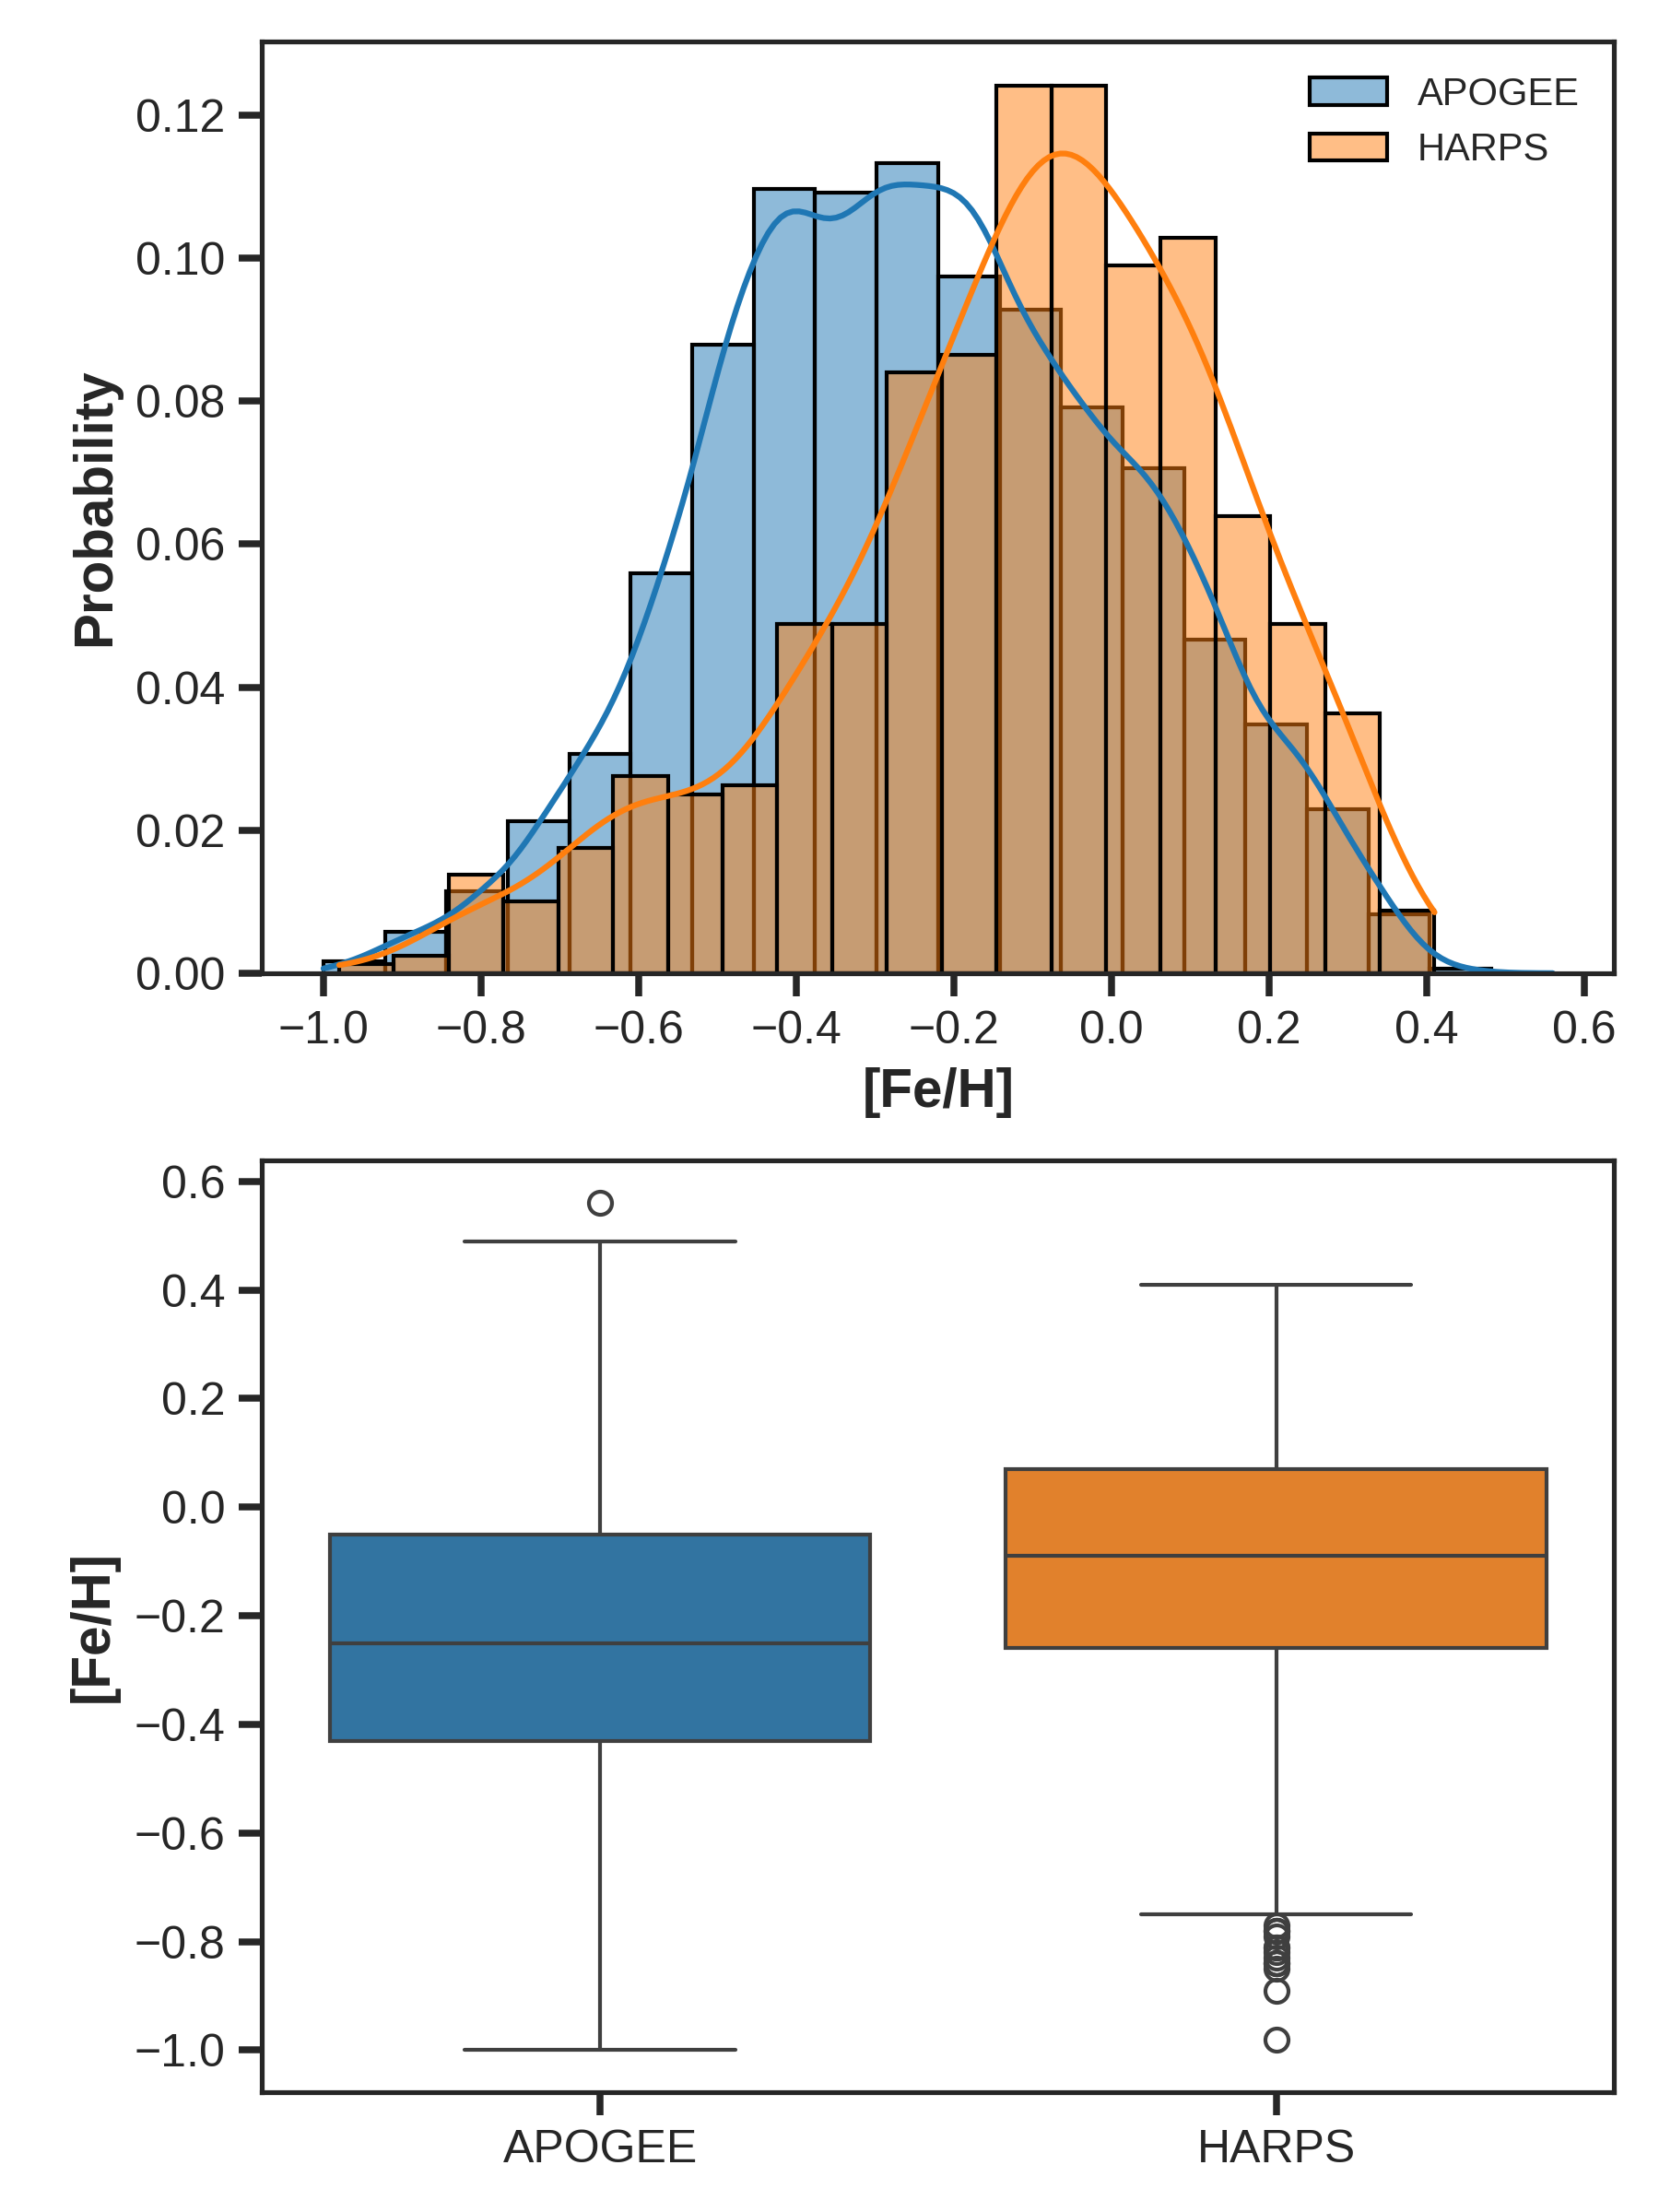
\includegraphics[width=1\linewidth]{feh_distributions_apogee_harps.png}
    \caption{
    Distributions of [Fe/H] for the two samples used in this work: APOGEE (blue)  and HARPS (green). The top panel shows the normalized probability density functions, while the bottom panel presents boxplots summarizing the median and spread of the [Fe/H] distributions.
    }
    \label{fig:feh_distributions}
\end{figure}


\section{Predicting metallicity from kinematics}


To predict stellar metallicity, [Fe/H], we initially considered 9 kinematic and orbital parameters. These include the Galactic velocity components  ($\mathrm{U_{LSR}}$, $\mathrm{V_{LSR}}$, and $\mathrm{W_{LSR}}$) and the total space velocity ($\mathrm{UVW_{LSR}} = \sqrt{U_{\rm LSR}^2 + V_{\rm LSR}^2 + W_{\rm LSR}^2}$
),  orbital parameters derived from orbit integration (the maximum vertical excursion $Z_{\max}$, the pericentric and apocentric distances $R_{\rm peri}$ and $R_{\rm apo}$  and the orbital eccentricity $e$), as well as the probability of belonging to the Galactic thin-disk population, $P_{\rm gal}$.

To quantify the statistical relationships between the kinematic properties and metallicity, we evaluated monotonic correlations using Spearman’s rank coefficient and nonlinear dependencies using mutual information (MI). MI quantifies the general statistical dependence between two variables, including nonlinear relationships, without assuming monotonicity or linearity. It therefore complements Spearman’s rank coefficient and allows us to identify features that may contain predictive information beyond simple monotonic trends.

Among all parameters, $Z_{\max}$ and $P_{\rm gal}$ show the strongest correlations with metallicity, but with opposite signs. The maximum vertical excursion $Z_{\max}$ exhibits a clear negative correlation, indicating that stars reaching larger distances from the Galactic plane tend to be more metal-poor. In contrast, the thin-disk membership probability $P_{\rm gal}$ correlates positively with [Fe/H], consistent with the higher metallicities characteristic of thin-disk stars.

While some quantitative differences are observed between the APOGEE and HARPS samples—reflecting their distinct stellar populations and selection functions—the overall trends remain consistent, with $Z_{\max}$ and $P_{\rm gal}$ emerging as the dominant kinematic predictors of metallicity.

To assess multicollinearity among the input features, we computed the variance inflation factor (VIF). Large VIF values indicate strong linear dependence among variables.

As expected, several parameters exhibit large VIF values. Interestingly, the two strongest predictors identified in the correlation analysis, $Z_{\max}$ and $P_{\rm gal}$, also display comparatively low VIF values, indicating that their predictive power is not merely a consequence of linear redundancy with other orbital parameters.

Although substantial multicollinearity is present (VIF $>$ 10 is typically considered as substantial), particularly among the derived velocity quantities, we retained all features in the subsequent analysis, as tree-based ensemble models are largely insensitive to correlated predictors. 

\section{Predicting individual abundances}

\section{Abundance ratios relevant for exoplanet research}

\section{Conclusion and summary}

%comparison between the surveys https://ui.adsabs.harvard.edu/abs/2023A%26A...670A.107H/abstract
%%%%%%%%%%%%%%%%%%%%%%%%%%%%%%%%%%%%%%%%%%%%%%%%%%%%%%%%%%%%%%
\begin{acknowledgements}
V.~A. acknowledges support from FCT – Funda\c{c}\~ao para a Ci\^encia e Tecnologia through national funds and from FEDER via COMPETE2020 – Programa Operacional Competitividade e Internacionalização, under the grants UIDB/04434/2020 (DOI: 10.54499/UIDB/04434/2020) and UIDP/04434/2020 (DOI: 10.54499/UIDP/04434/2020), as well as through a work contract funded by the FCT Scientific Employment Stimulus program (reference 2023.06055.CEECIND/CP2839/CT0005, DOI: 10.54499/2023.06055.CEECIND/CP2839/CT0005).
\end{acknowledgements}




%%%%%%%%%%%%%%%%%%%%%%%%%%%%%%%%%%%%%%%%%%%%%%%%%%%%%%%%%%%%%%
% WARNING
% Please note that we have included the references below in
% order to compile the document, but we ask you to:
%
% - use BibTeX with the regular commands:
\bibliographystyle{aa} % style aa.bst
\bibliography{references} % your references Yourfile.bib


%%%%%%%%%%%%%%%%%%%%%%%%%%%%%%%%%%%%%%%%%%%%%%%%%%%%%%%%%%%%%%%
% Appendices must be placed after   \end{thebibliography}
% They will be placed automatically on a new page.
%%%%%%%%%%%%%%%%%%%%%%%%%%%%%%%%%%%%%%%%%%%%%%%%%%%%%%%%%%%%%%%
\begin{appendix}

\section{Construction of the samples} \label{target_selection}

In this section, we describe in detail the selection criteria adopted for the different samples and the determination of the relevant parameters.

\subsection{APOGEE DR17}

For the APOGEE sample, we performed a careful quality selection to ensure reliable stellar parameters and elemental abundances. We excluded stars with problematic \texttt{APOGEE\_STARFLAG} entries, removing objects affected by high persistence (\texttt{PERSIST\_HIGH}, bit~9), low signal-to-noise ratio (\texttt{LOW\_SNR}, bit~4), contamination from a very bright neighbor (\texttt{VERY\_BRIGHT\_NEIGHBOR}, bit~3), and spectra showing significant positive or negative persistence jumps in the blue chip (\texttt{PERSIST\_JUMP\_POS}, bit~12; \texttt{PERSIST\_JUMP\_NEG}, bit~13). We also excluded stars flagged as having inconsistent radial velocity determinations (\texttt{SUSPECT\_RV\_COMBINATION}, bit~16).

To ensure a homogeneous and representative dataset, we selected only stars belonging to the main APOGEE survey by requiring \texttt{EXTRATARG}~=~0, thereby excluding ancillary and calibration targets. Using the \texttt{PROGRAMNAME} flag, we further removed stars that were part of minor programs (those containing fewer than 1500 stars) targeting specific objects.

To guarantee robust stellar parameters, elemental abundances, and kinematic measurements, we applied the following additional selection criteria \citep[see e.g.,][]{Feltzing-23}: 
we retained only red giant stars with effective temperatures $4000 < T_{\mathrm{eff}} < 6000$~K, surface gravities $1.0 < \log g < 2.5$~dex, and spectra with signal-to-noise ratios $\mathrm{S/N} > 100$. We required that \texttt{FE\_H\_FLAG}~=~0 and \texttt{X\_FE\_FLAG}~=~0 for the key elements C, O, Mg, Si, and Fe, and that the uncertainties in the corresponding abundances be smaller than 0.05~dex. We further required relative parallax uncertainties $\sigma_\pi / \pi < 0.1$ to ensure reliable distances. 

Because the main motivation of the present work is to predict metallicities and abundances of exoplanet host stars, we restricted the sample to stars within the metallicity range $-1.0 < [\mathrm{Fe/H}] < 0.6$~dex. The upper limit was imposed to avoid unrealistically high values or chemically peculiar objects. We also verified that all selected stars possess measured radial velocities, \textit{Gaia} parallaxes, and proper motions, which were used to compute the kinematic properties of the sample.

After applying all the above selection criteria, the final APOGEE sample consists of about 46\,000 red giant stars.

%\subsection{GALAH DR4}

%Similar to the APOGEE sample, we also restricted the GALAH sample to stars with the most reliable stellar parameters and abundance determinations. We excluded stars with identified issues in their stellar parameter derivations by requiring \texttt{flag\_sp}~=~0. Only high-quality spectra were retained by selecting stars with \texttt{snr\_px\_ccd2}~$>$~50, corresponding to the SNR per pixel from the second GALAH camera. 

%We further limited the sample to FGK dwarf stars with  $5000 < T_{\mathrm{eff}} < 6300$~K and  $4.1 < \log g < 4.7$~dex. We required the metallicity and all relevant elemental abundance flags to be zero (e.g. \texttt{flag\_mg\_fe}~=~0), and the uncertainties in the abundances to be smaller than 0.1~dex. The metallicity range was restricted to $-1.0 < [\mathrm{Fe/H}] < 0.6$~dex to avoid metal-poor and chemically peculiar stars. 

%It is worth noting that the reported uncertainties in the GALAH abundances are systematically larger, as they account for both precision and accuracy effects \citep{Buder-25}. As for the APOGEE sample, we required relative parallax uncertainties $\sigma_\pi / \pi < 0.1$ to ensure reliable distance estimates.

%After applying all the above selection criteria, the final GALAH sample consists of approximately 71\,000 FGK dwarf stars.


\subsection{HARPS}

The HARPS sample consists of 798 FGK-type dwarf stars with homogeneously derived atmospheric parameters and elemental abundances \citep{Adibekyan-12, DelgadoMena-21}. The astrometric data for these stars were taken from \textit{Gaia}~DR3, and as for the other samples, we required relative parallax uncertainties $\sigma_\pi / \pi < 0.1$ to ensure reliable distances. 

The metallicities of the HARPS stars span the range $-1.0 < [\mathrm{Fe/H}] < 0.4$~dex. This sample, composed primarily of bright, nearby stars observed in the context of exoplanet searches, provides high-precision spectroscopic abundances and serves as an excellent benchmark for testing the machine learning models.


\subsection{Kinematics and dynamics of the stars}

Using the formulation of \citet{Johnson-87}, and combining the astrometric parameters and radial velocities of the stars, we computed the Galactic space velocity components ($U_{\mathrm{LSR}}$, $V_{\mathrm{LSR}}$, and $W_{\mathrm{LSR}}$) relative to the Local Standard of Rest (LSR). The solar motion with respect to the LSR was adopted from \citet{Schonrich-10}. 

We then estimated the probability of each star belonging to one of the three main Galactic stellar populations (the thin disk, thick disk, or halo) following the prescription of \citet{Reddy-06}. This method assumes that stars in the solar neighborhood can be described as a mixture of these three kinematic populations, each characterized by Gaussian velocity distributions in the $U$, $V$, and $W$ components \citep{Schwarzschild-1907}. 

To further characterize the stellar orbits, we used the \texttt{galpy} package \citep{Bovy-15} to compute orbital parameters within a realistic Milky Way gravitational potential. For each star, we derived the pericentric ($R_{\mathrm{peri}}$) and apocentric ($R_{\mathrm{apo}}$) distances, orbital eccentricity ($e$), and the maximum vertical distance from the Galactic plane ($Z_{\mathrm{max}}$). The orbit integration was carried out assuming the \texttt{MWPotential2014} model provided by \texttt{galpy}, integrating each orbit over several Galactic rotations. 

These quantities provide insight into the dynamical behavior and population membership of the stars, and the methodology has been extensively applied in previous works \citep[e.g.,][]{Adibekyan-12}.



\section{Exploratory data analysis for metallicity determination}

In this section, we provide the detailed results of the exploratory data analysis (EDA) performed to characterize the statistical relationships between the selected parameters and stellar metallicity.


\subsection{Spearman rank correlation analysis}

We computed Spearman’s rank correlation coefficient $\rho$ between each kinematic feature and [Fe/H] separately for the APOGEE and HARPS samples. Spearman’s coefficient measures monotonic associations without assuming linearity.

Figure~\ref{fig:spearman_appendix} presents the full set of correlation coefficients. In both samples, $Z_{\max}$ exhibits the strongest negative correlation with metallicity, while $P_{\rm gal}$ shows the strongest positive correlation. The next most correlated parameters are the orbital eccentricity $e$ and the total space velocity $\mathrm{UVW_{LSR}}$.

Although the absolute values of the coefficients differ slightly between APOGEE and HARPS—likely due to differences in stellar populations and sample size—the overall ranking of highly correlated features remains consistent.

\begin{figure*}
    \centering
    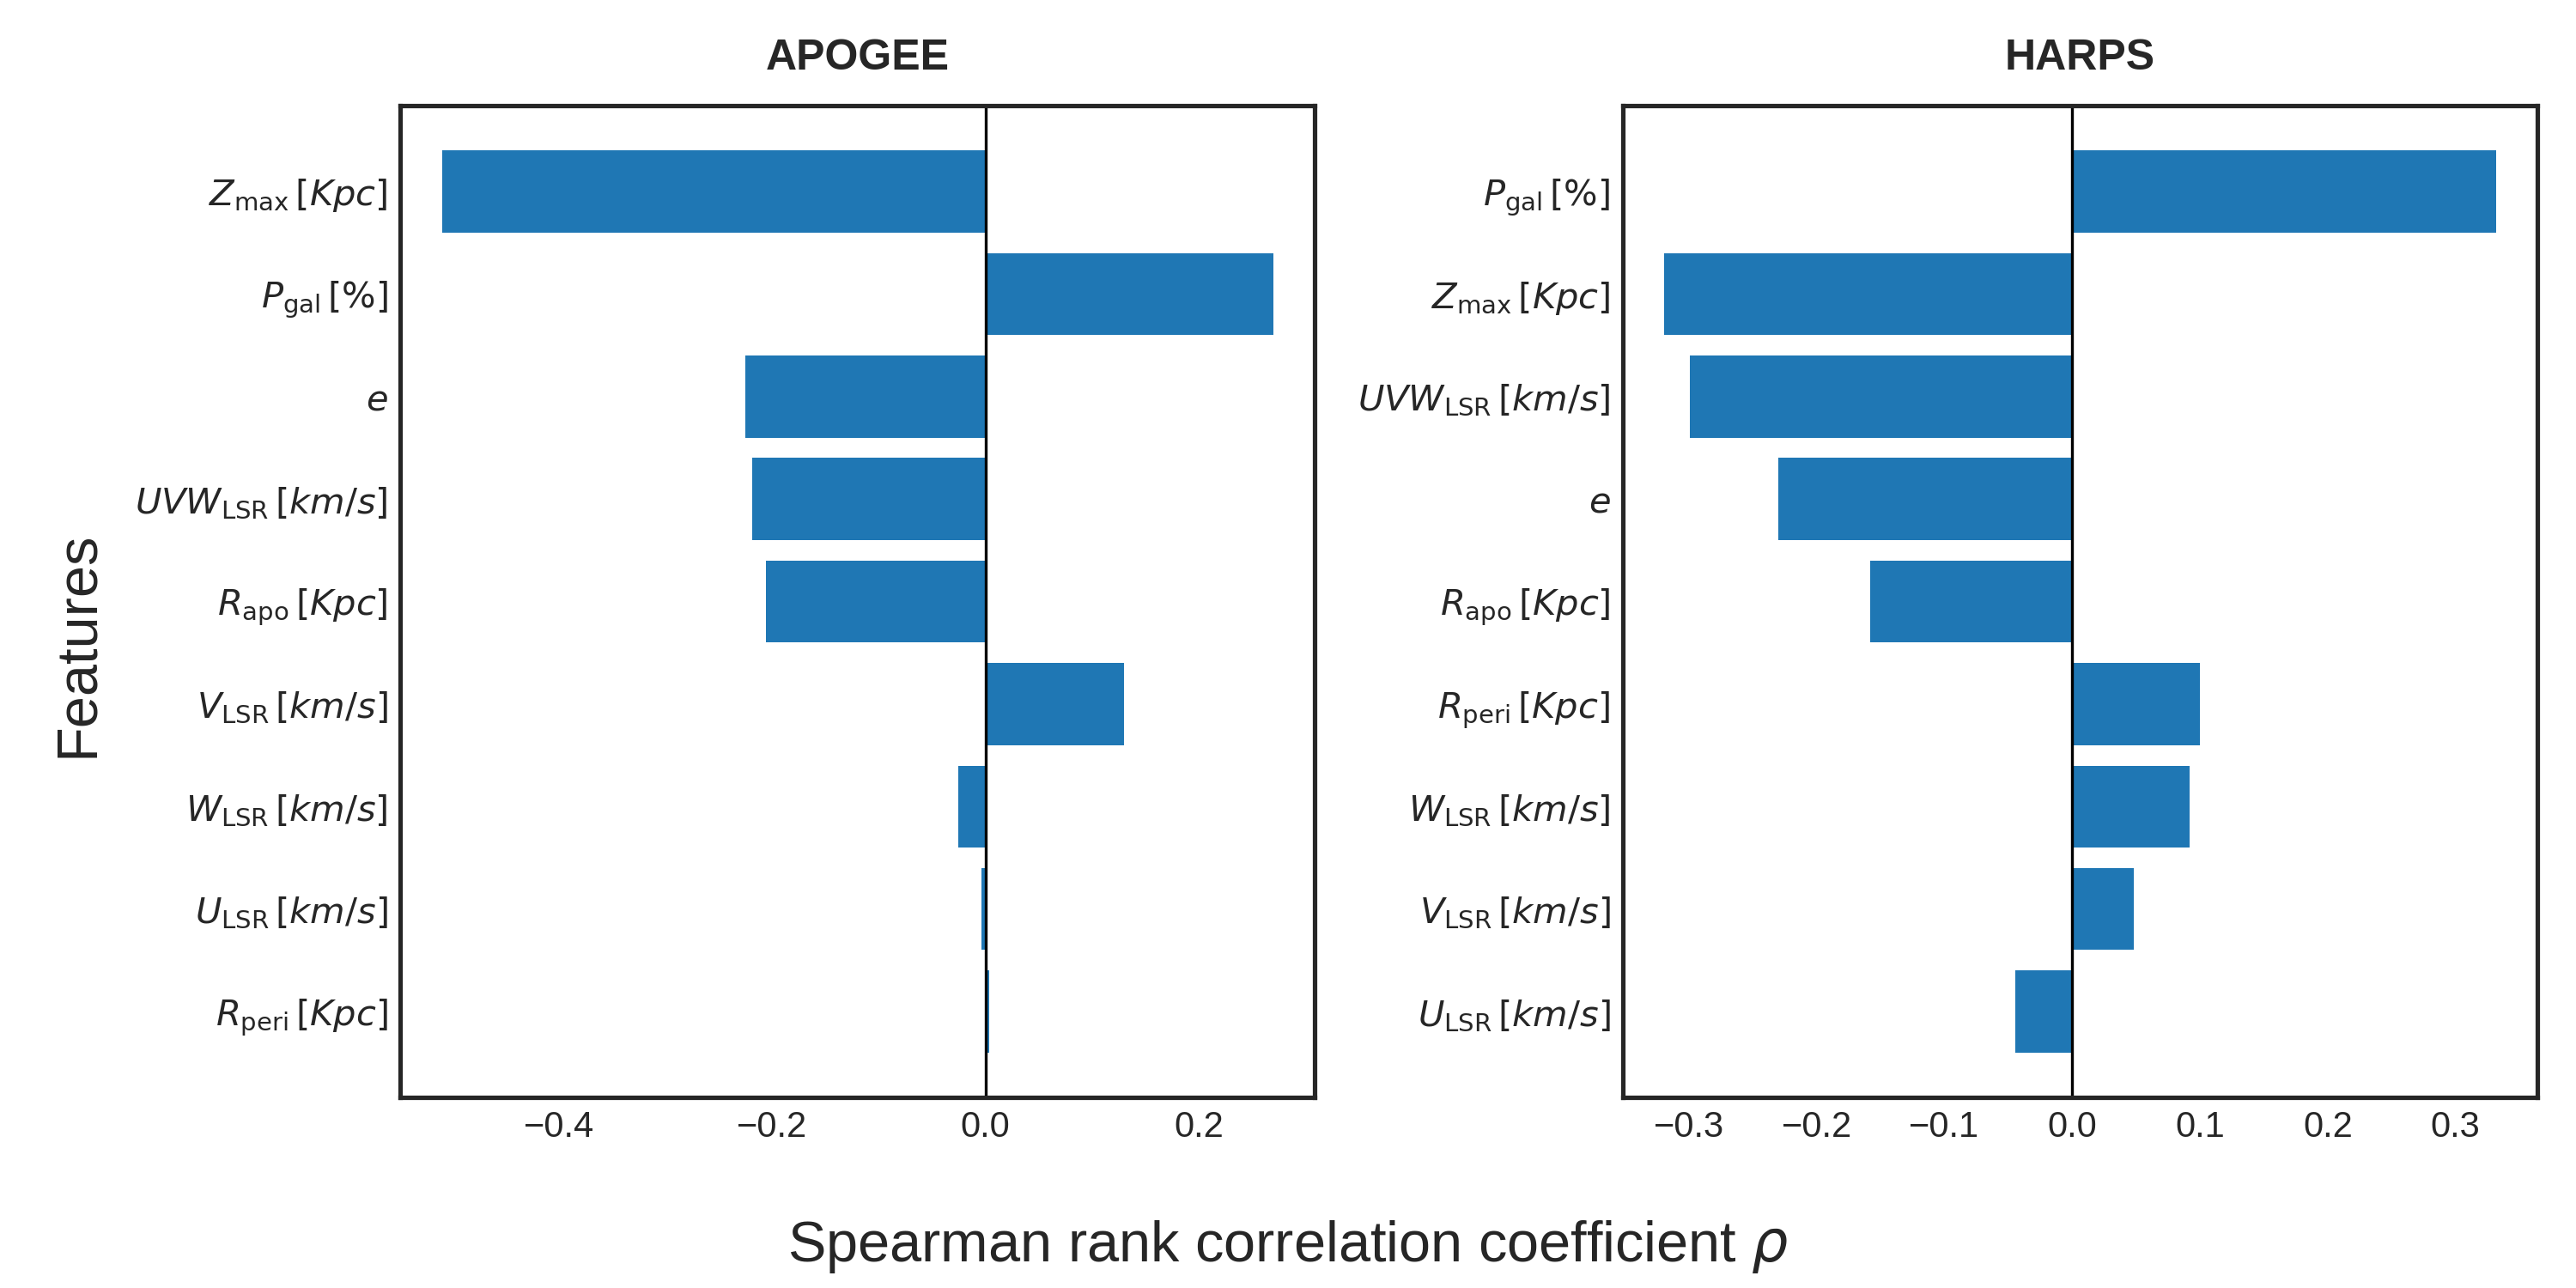
\includegraphics[width=1\textwidth]{correlations.png}
    \caption{Spearman rank correlation coefficients between the parameters and [Fe/H] for the APOGEE (left) and HARPS (right) samples.}
    \label{fig:spearman_appendix}
\end{figure*}


\subsection{Mutual information analysis}

To quantify nonlinear dependencies between the kinematic parameters and metallicity, we computed the mutual information (MI) between each feature and [Fe/H]. MI captures general statistical dependence, including nonlinear relationships.

To quantify nonlinear dependencies between the kinematic parameters and metallicity,
we computed the mutual information (MI) between each feature and [Fe/H].
Mutual information measures the general statistical dependence between two variables. Unlike correlation coefficients, MI does not assume linearity or monotonicity and is sensitive to arbitrary nonlinear relationships.

An MI value of zero indicates statistical independence, while larger values imply stronger dependence. In this work, MI was estimated using a non-parametric k-nearest-neighbour approach (with $k$ = 3), which is well suited for continuous variables.


The MI values for both samples are shown in Figure~\ref{fig:mi_appendix}. Consistent with the correlation analysis, $Z_{\max}$ and $P_{\rm gal}$ (also eccentricity) contain the largest amount of predictive information.

In addition, parameters such as $R_{\rm peri}$ show enhanced importance in the MI analysis compared to its rank correlation, suggesting the presence of nonlinear contributions to the metallicity-kinematics relation.

\begin{figure*}
    \centering
    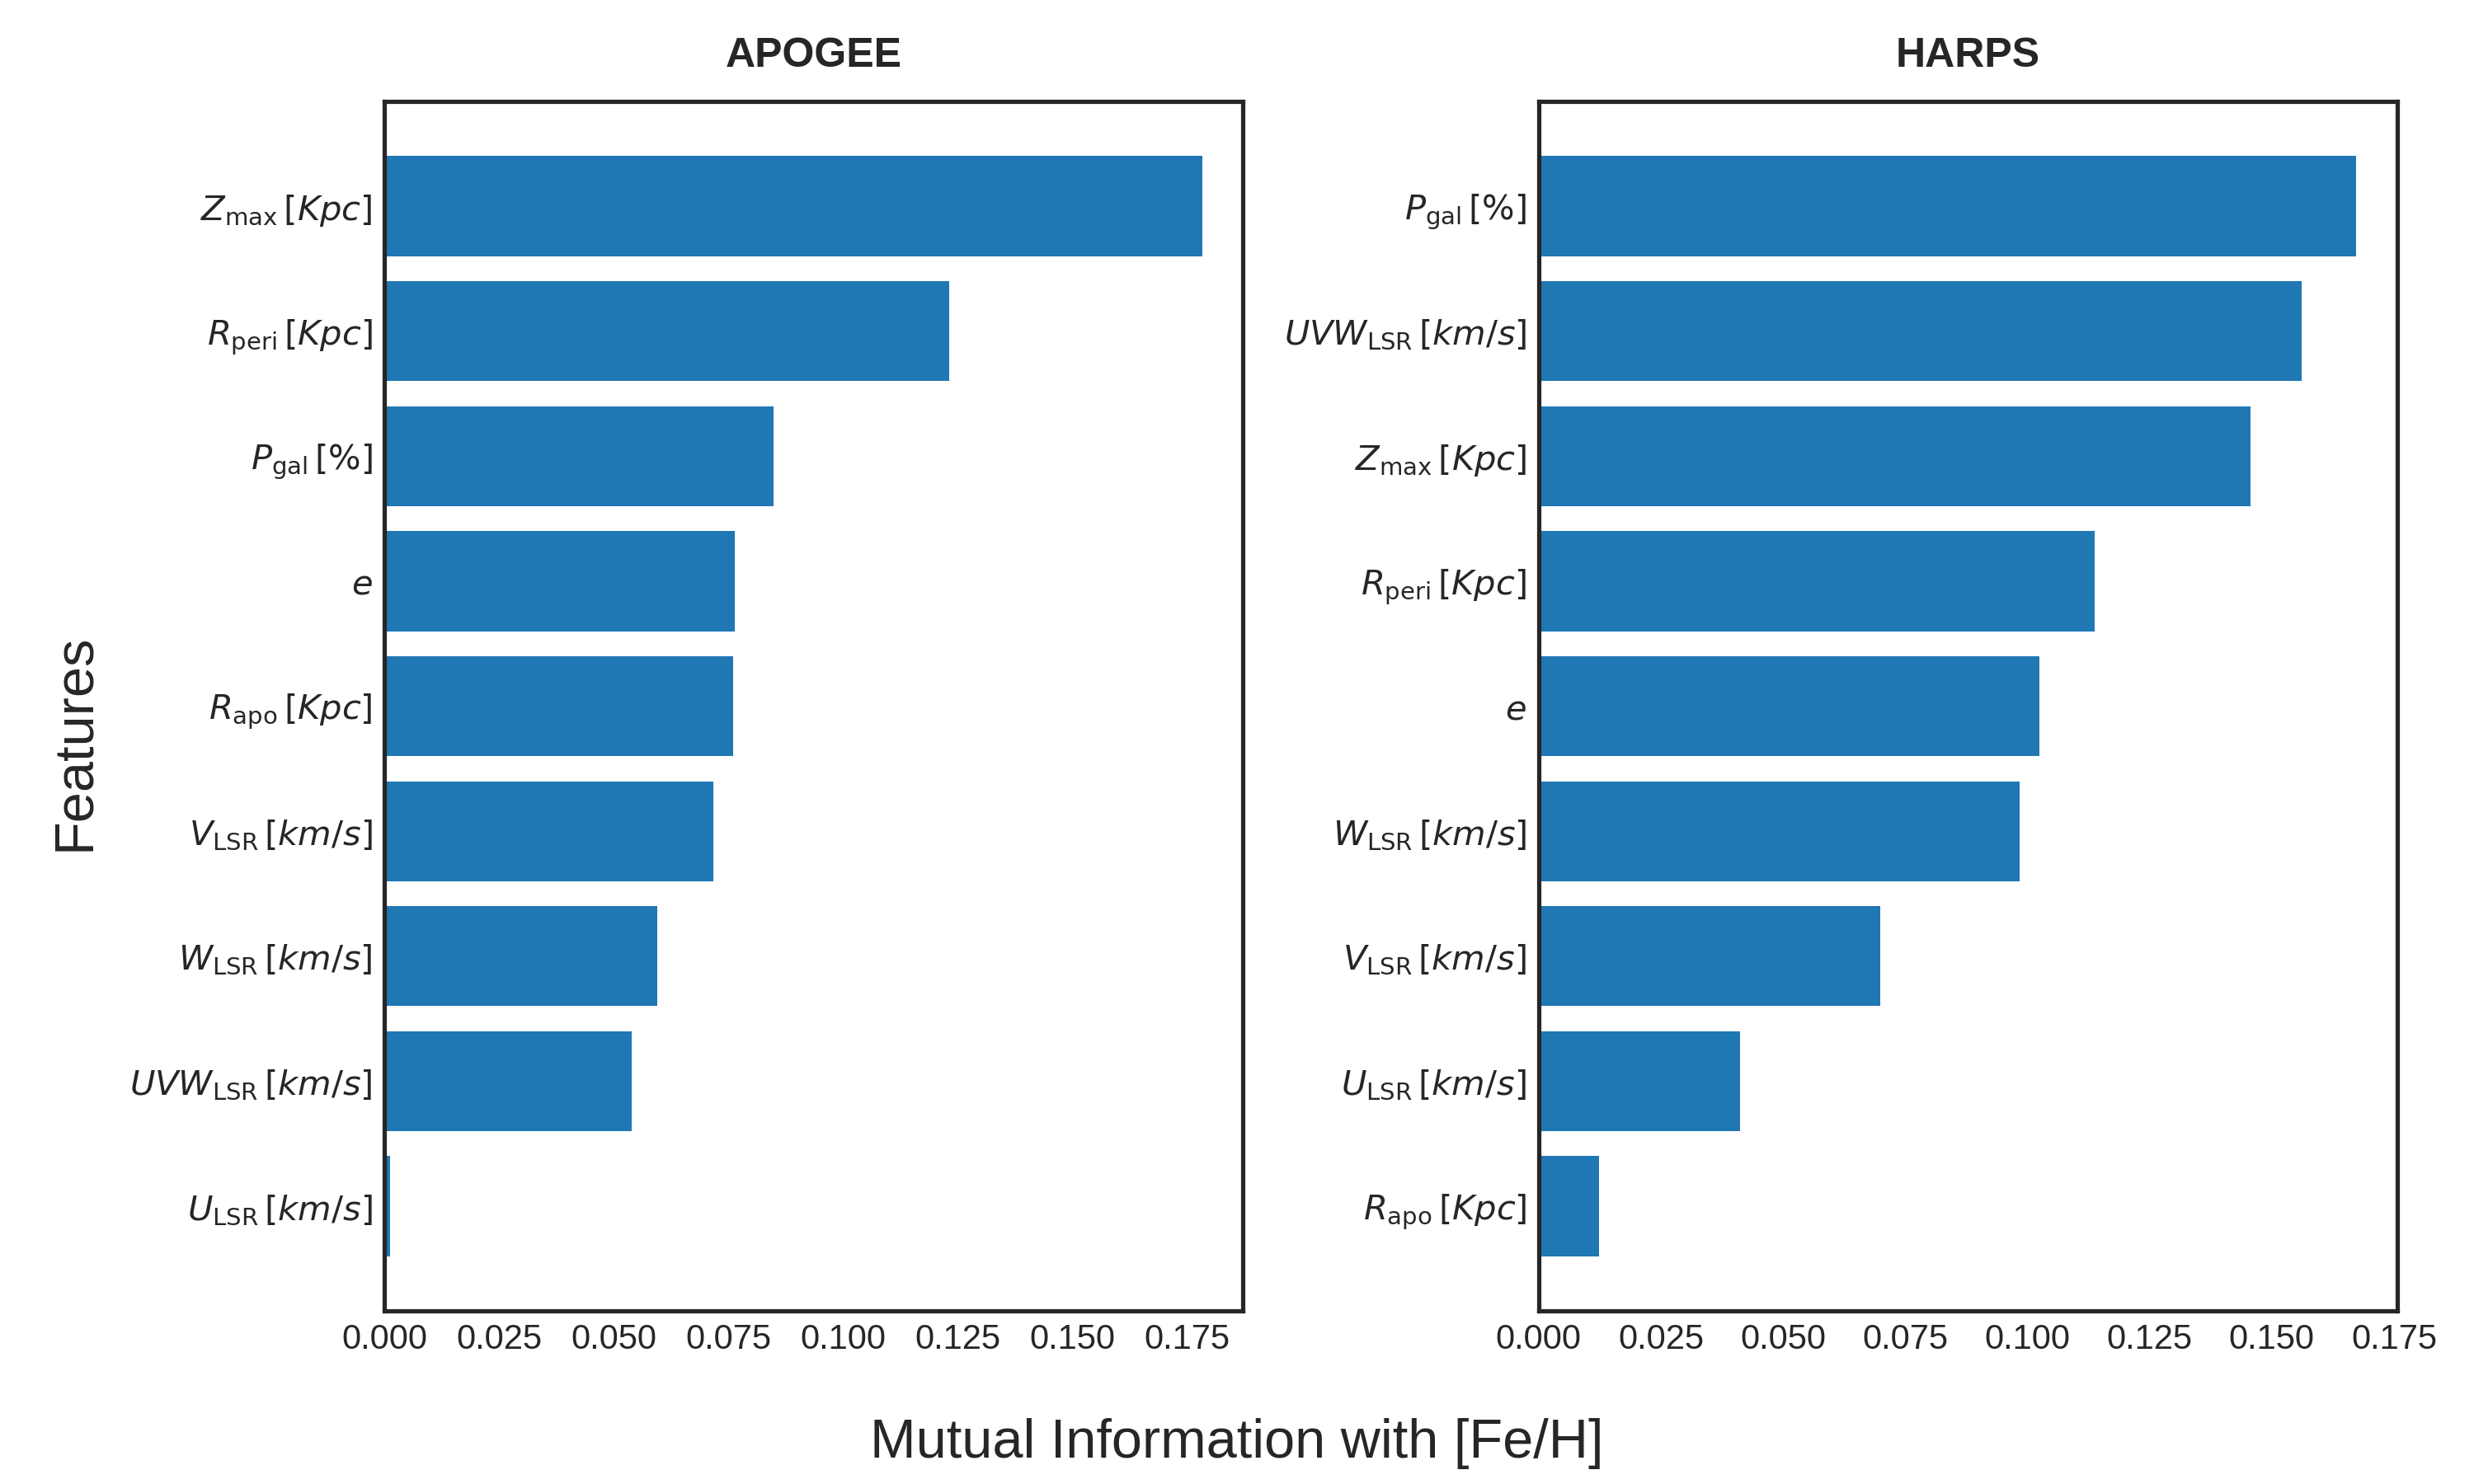
\includegraphics[width=1\textwidth]{MI.png}
    \caption{Mutual information between kinematic parameters and [Fe/H] for the APOGEE (left) and HARPS (right) samples.}
    \label{fig:mi_appendix}
\end{figure*}


\subsection{Multicollinearity diagnostics}

We evaluated multicollinearity among the predictors using the variance inflation factor (VIF), defined as
\begin{equation}
\mathrm{VIF}_j = \frac{1}{1 - R_j^2},
\end{equation}
where $R_j^2$ is obtained by regressing feature $j$ against all remaining predictors. The VIF quantifies how much the variance of a regression coefficient is inflated due to linear dependence among input variables.

A VIF value of 1 indicates no multicollinearity, values between 1 and 5 are generally considered mild, values above 5 indicate moderate collinearity, and values exceeding 10 are typically interpreted as substantial multicollinearity.

High multicollinearity can lead to unstable coefficient estimates and inflated variance in linear models. However, its impact depends on the nature of the predictive algorithm. Tree-based ensemble methods, which perform recursive partitioning rather than coefficient estimation, are generally more robust to correlated predictors.

The resulting VIF values are shown in Figure~\ref{fig:vif_appendix}. As expected, several parameters exhibit large VIF values due to their deterministic dependence on the other parameters. $Z_{\max}$ and $P_{\rm gal}$ display comparatively lower VIF values, indicating that they are not strongly linearly redundant with the remaining parameters.

\begin{figure*}
    \centering
    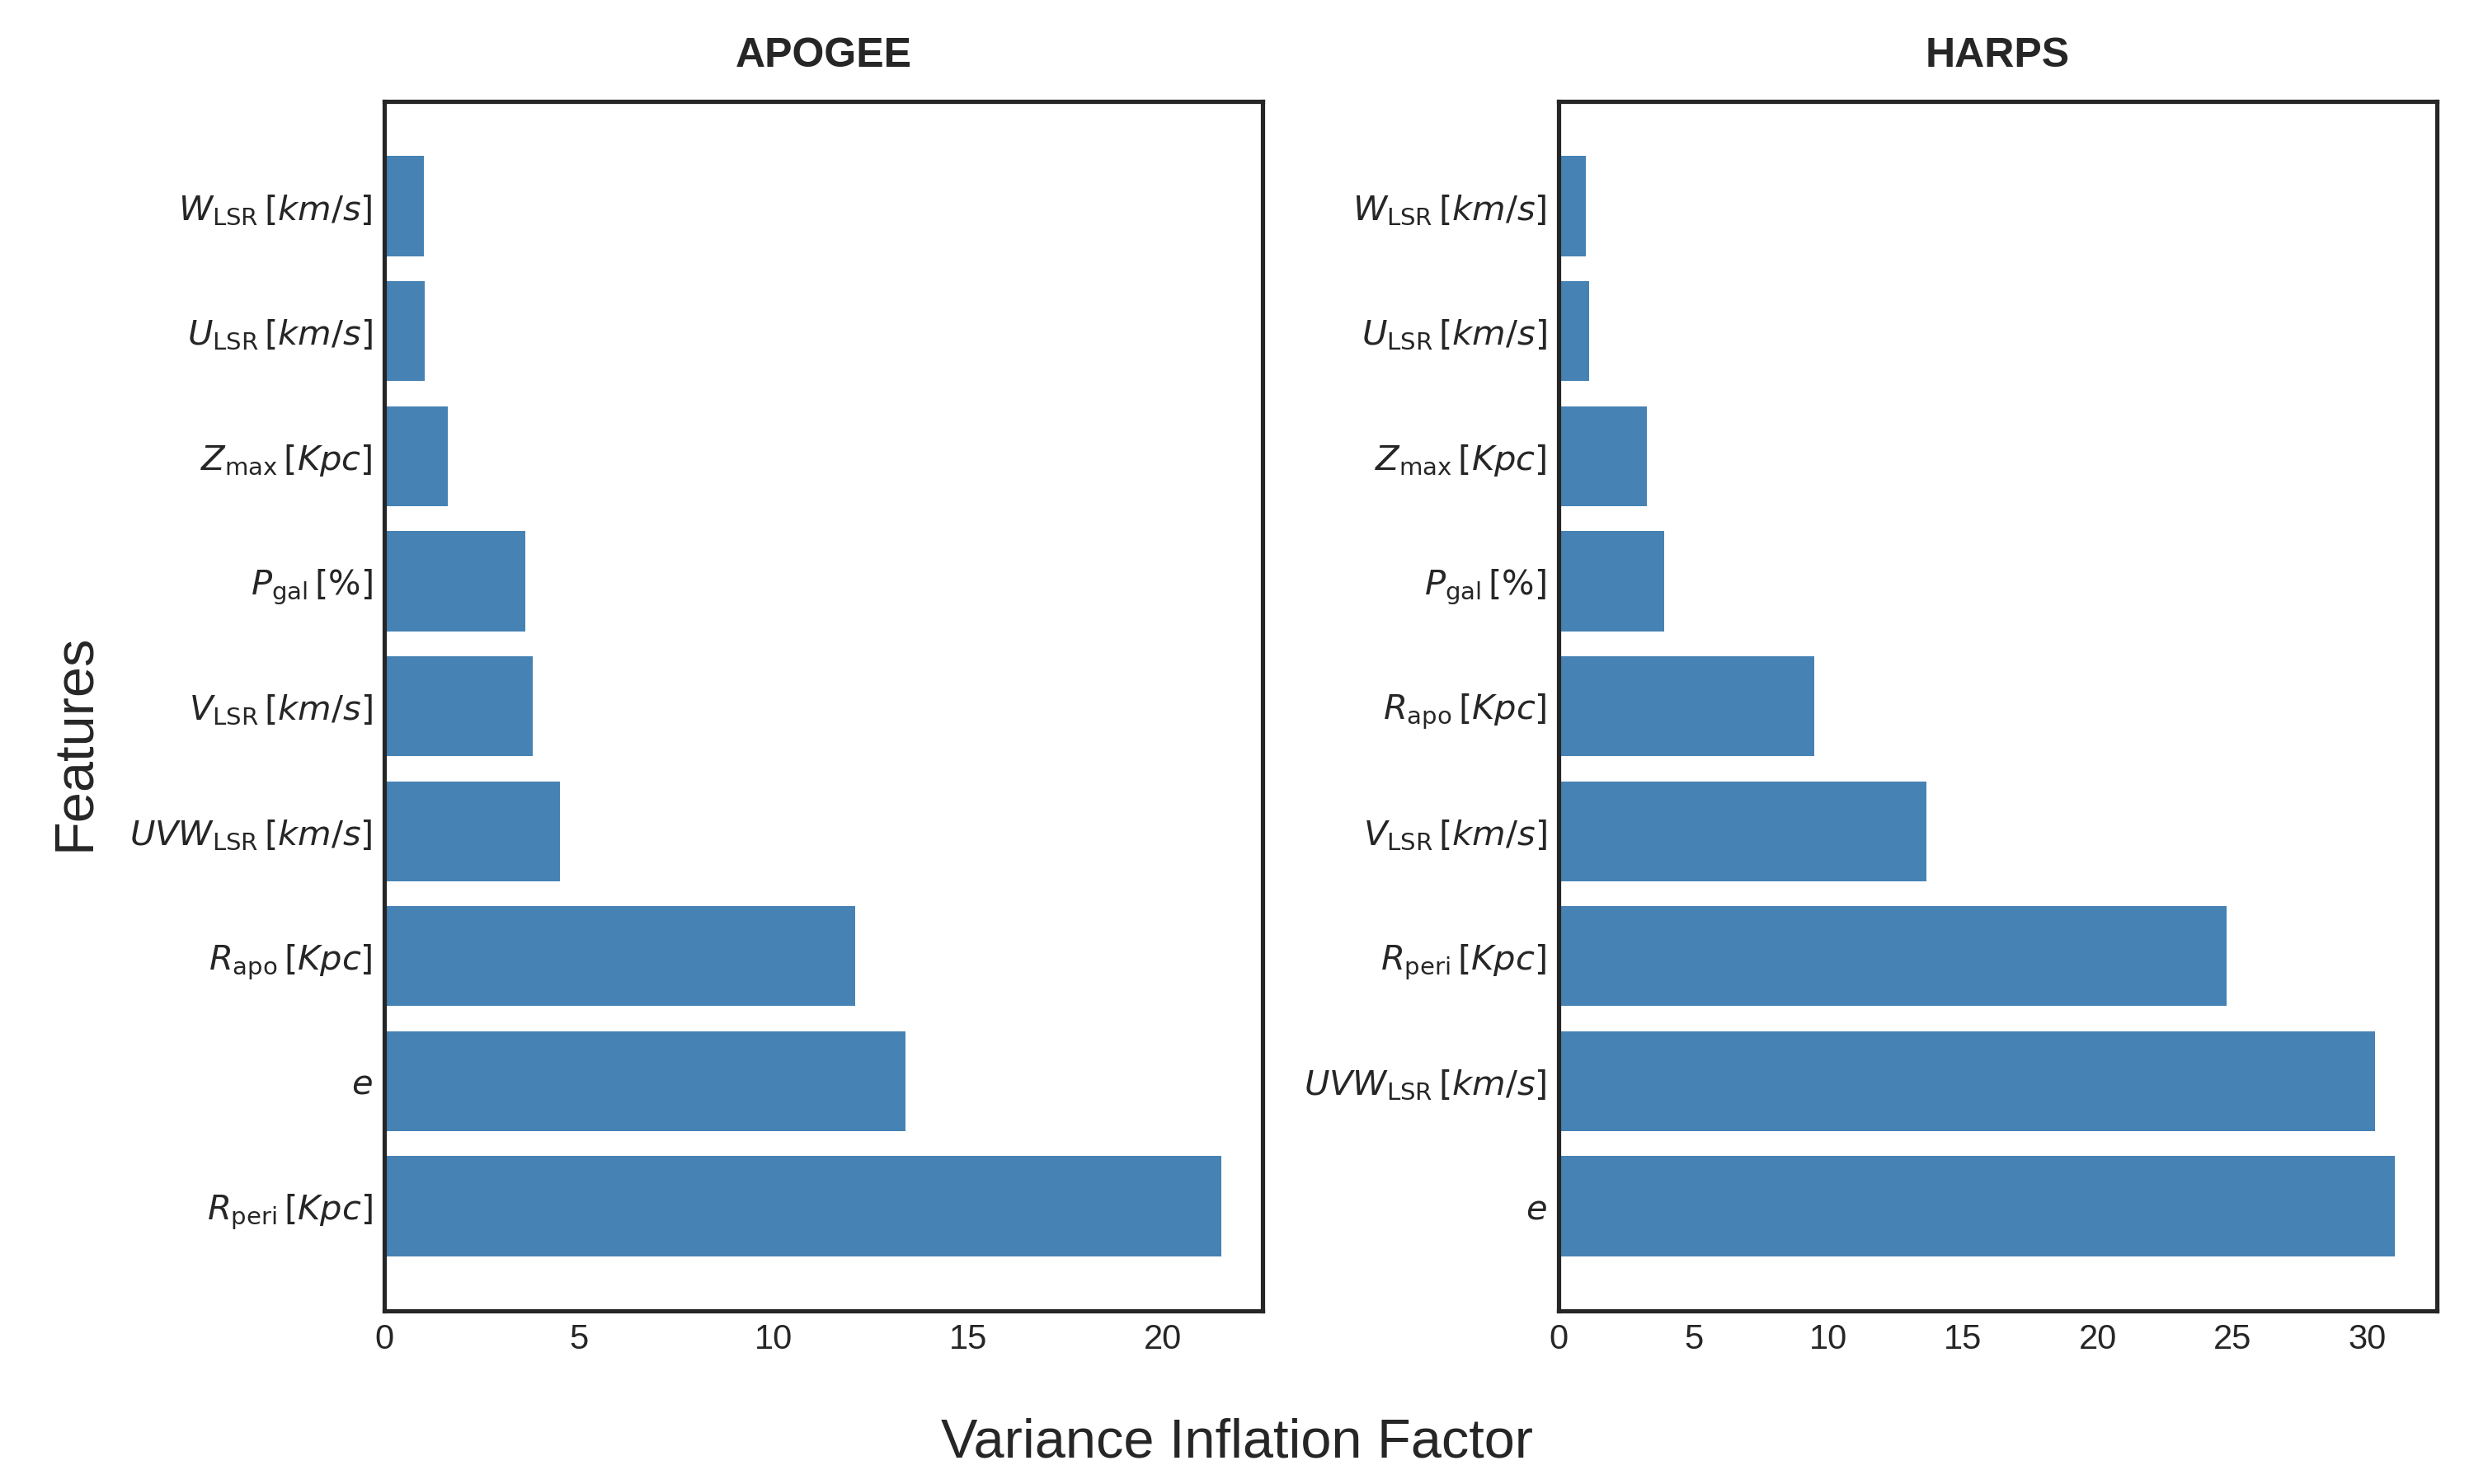
\includegraphics[width=1\textwidth]{VIF.png}
    \caption{Variance inflation factors (VIF) for the kinematic parameters in the APOGEE (left) and HARPS (right) samples.}
    \label{fig:vif_appendix}
\end{figure*}



\subsection{Comparison of parameter distributions}

Figure~\ref{fig:feature_distributions} presents the distributions of the kinematic and orbital parameters for the APOGEE and HARPS samples. The upper panels show probability-normalized histograms, while the lower panels display boxplots summarizing the median and spread of each parameter.

Some differences are observed between the two samples. The HARPS dataset, composed primarily of nearby solar-type dwarf stars, is confined to a relatively narrow range of velocities and orbital parameters, reflecting its local nature and selection for exoplanet surveys.
In contrast, the APOGEE red giant sample spans a significantly broader range in velocity space and orbital properties, including larger values of $Z_{\max}$, eccentricity, and total space velocity $\mathrm{UVW_{LSR}}$, consistent with its wider spatial coverage across different Galactic environments.

Despite these differences in dispersion, the APOGEE sample largely encompasses the parameter range covered by HARPS. This overlap ensures that the machine-learning models trained on APOGEE data operate within the dynamical regime relevant for the local HARPS stars, while also capturing a broader diversity of Galactic populations.

\begin{figure*}
\centering
\begin{subfigure}{0.32\textwidth}
    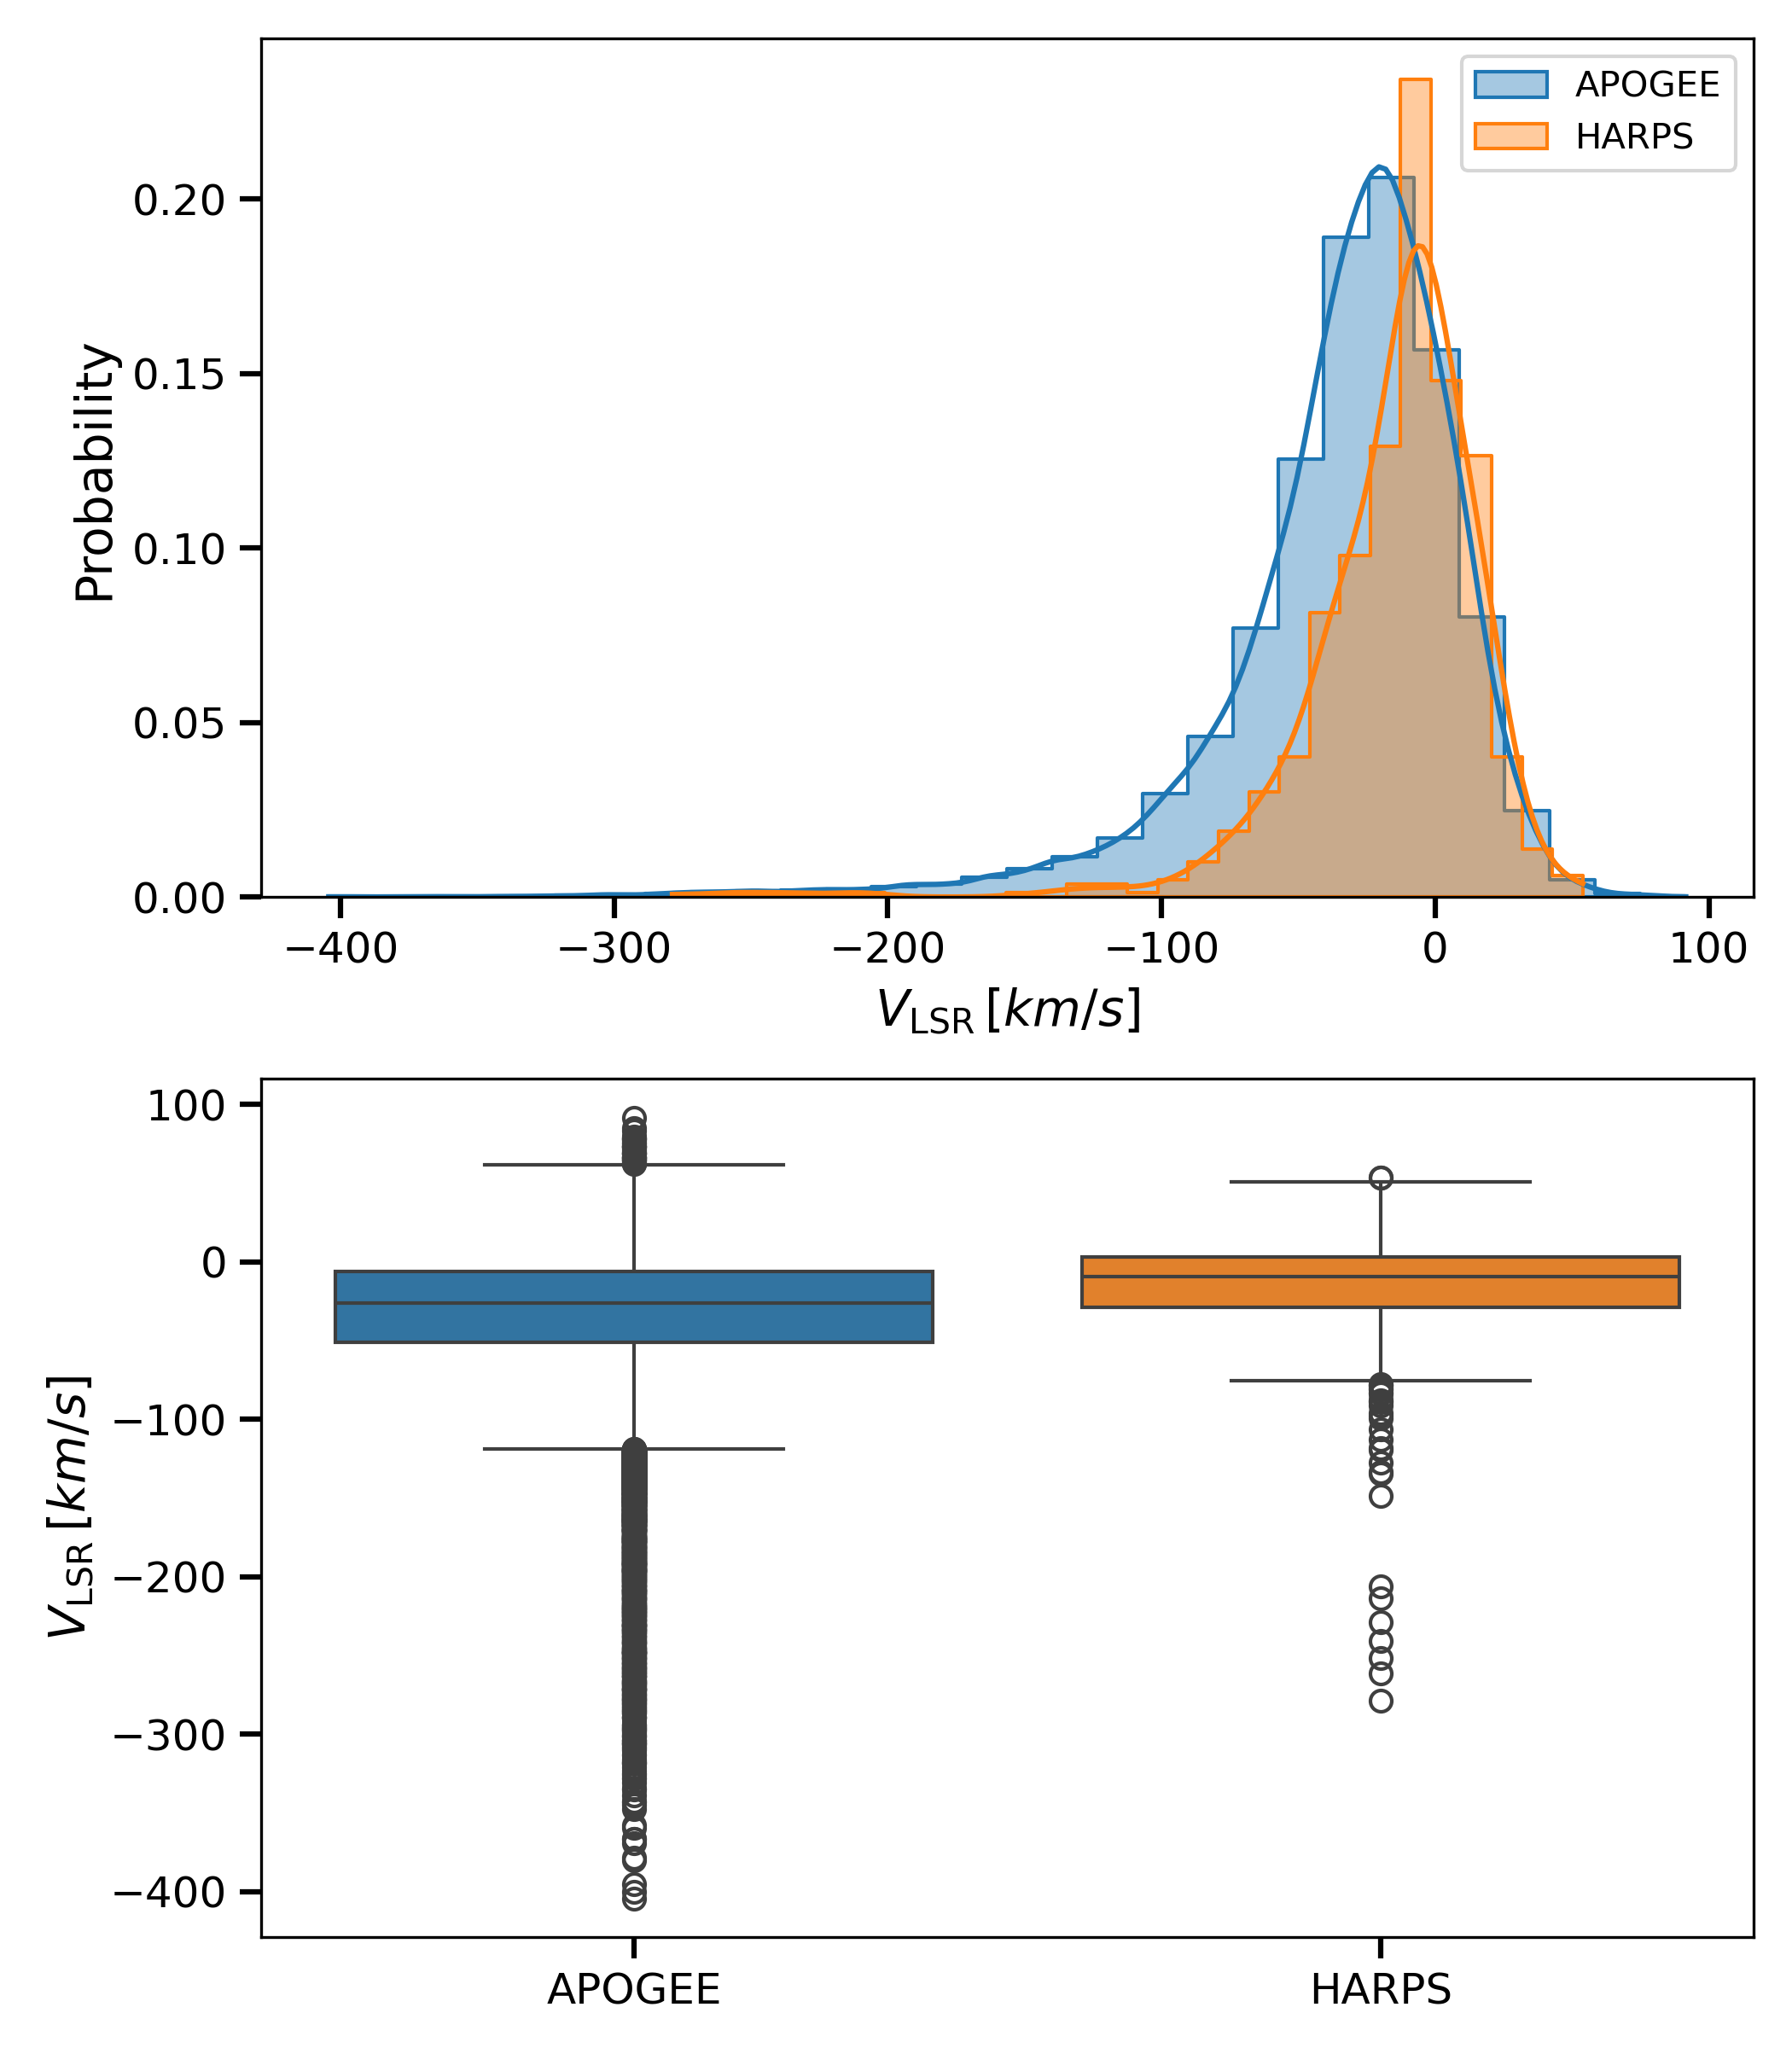
\includegraphics[width=\linewidth]{figures/dist_V_lsr.png}
    \caption{$V_{\mathrm{LSR}}\, [km/s]$}
\end{subfigure}
\hfill
\begin{subfigure}{0.32\textwidth}
    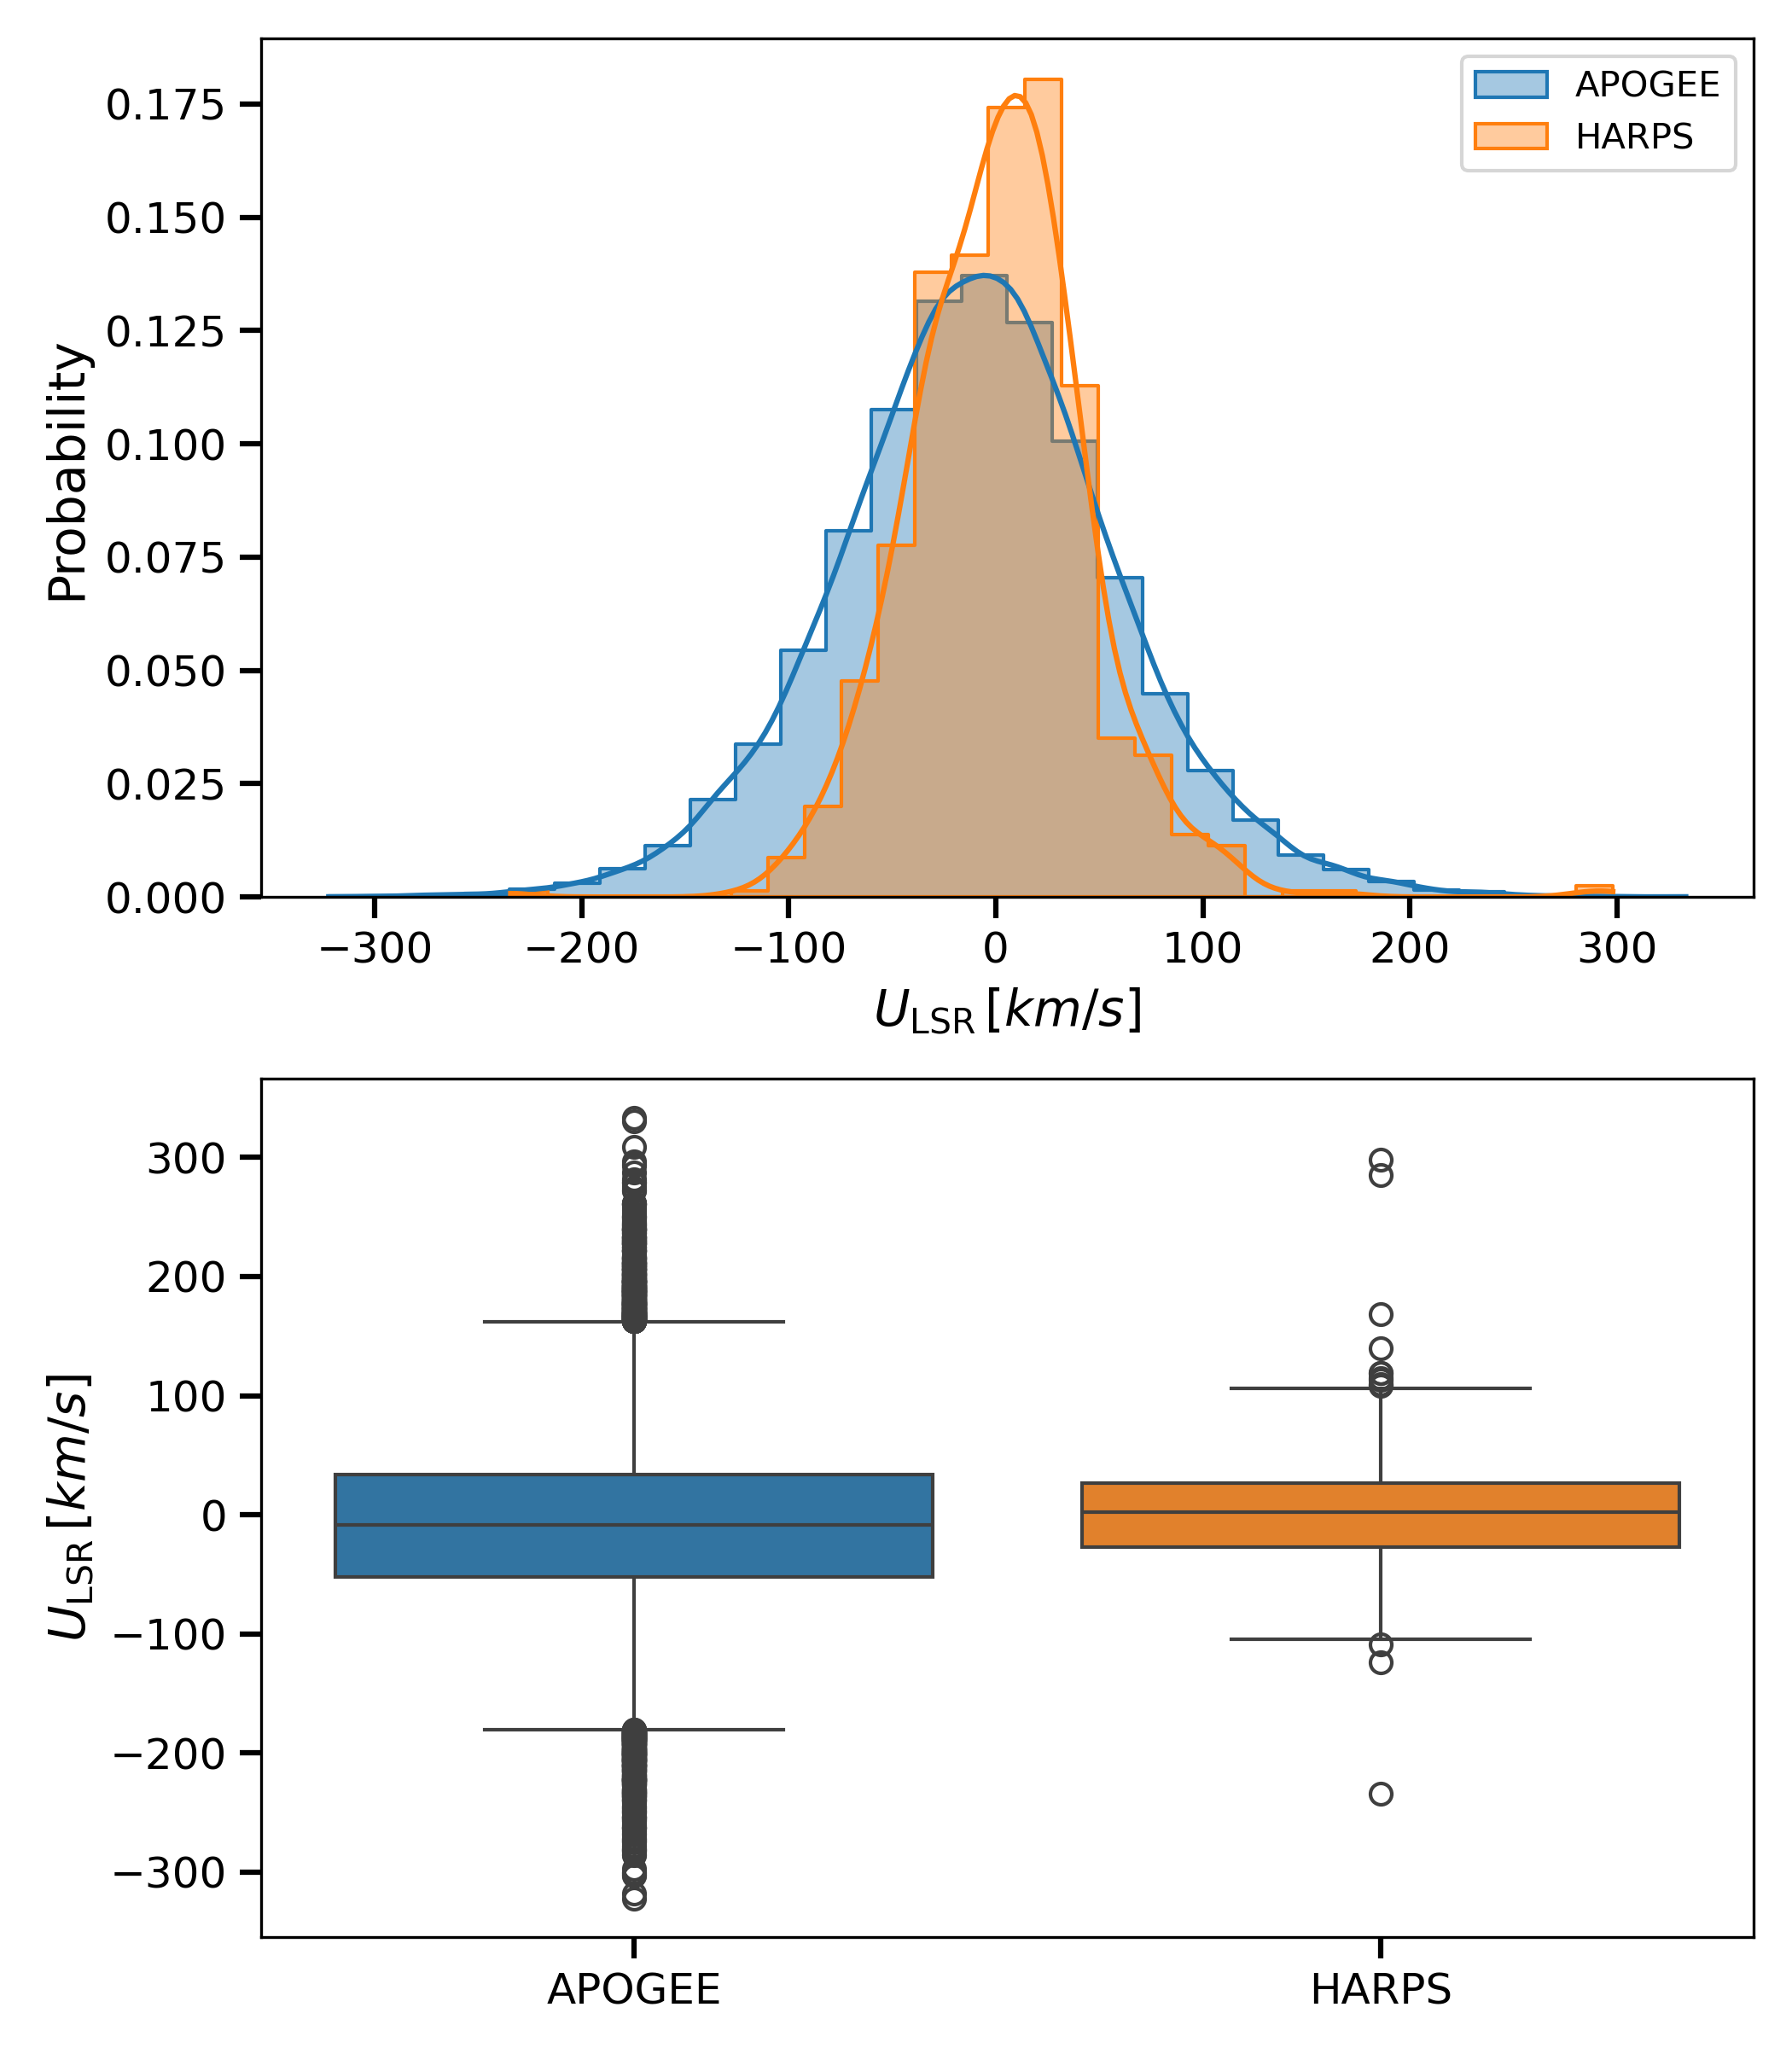
\includegraphics[width=\linewidth]{figures/dist_U_lsr.png}
    \caption{$U_{\mathrm{LSR}}\, [km/s]$}
\end{subfigure}
\hfill
\begin{subfigure}{0.32\textwidth}
    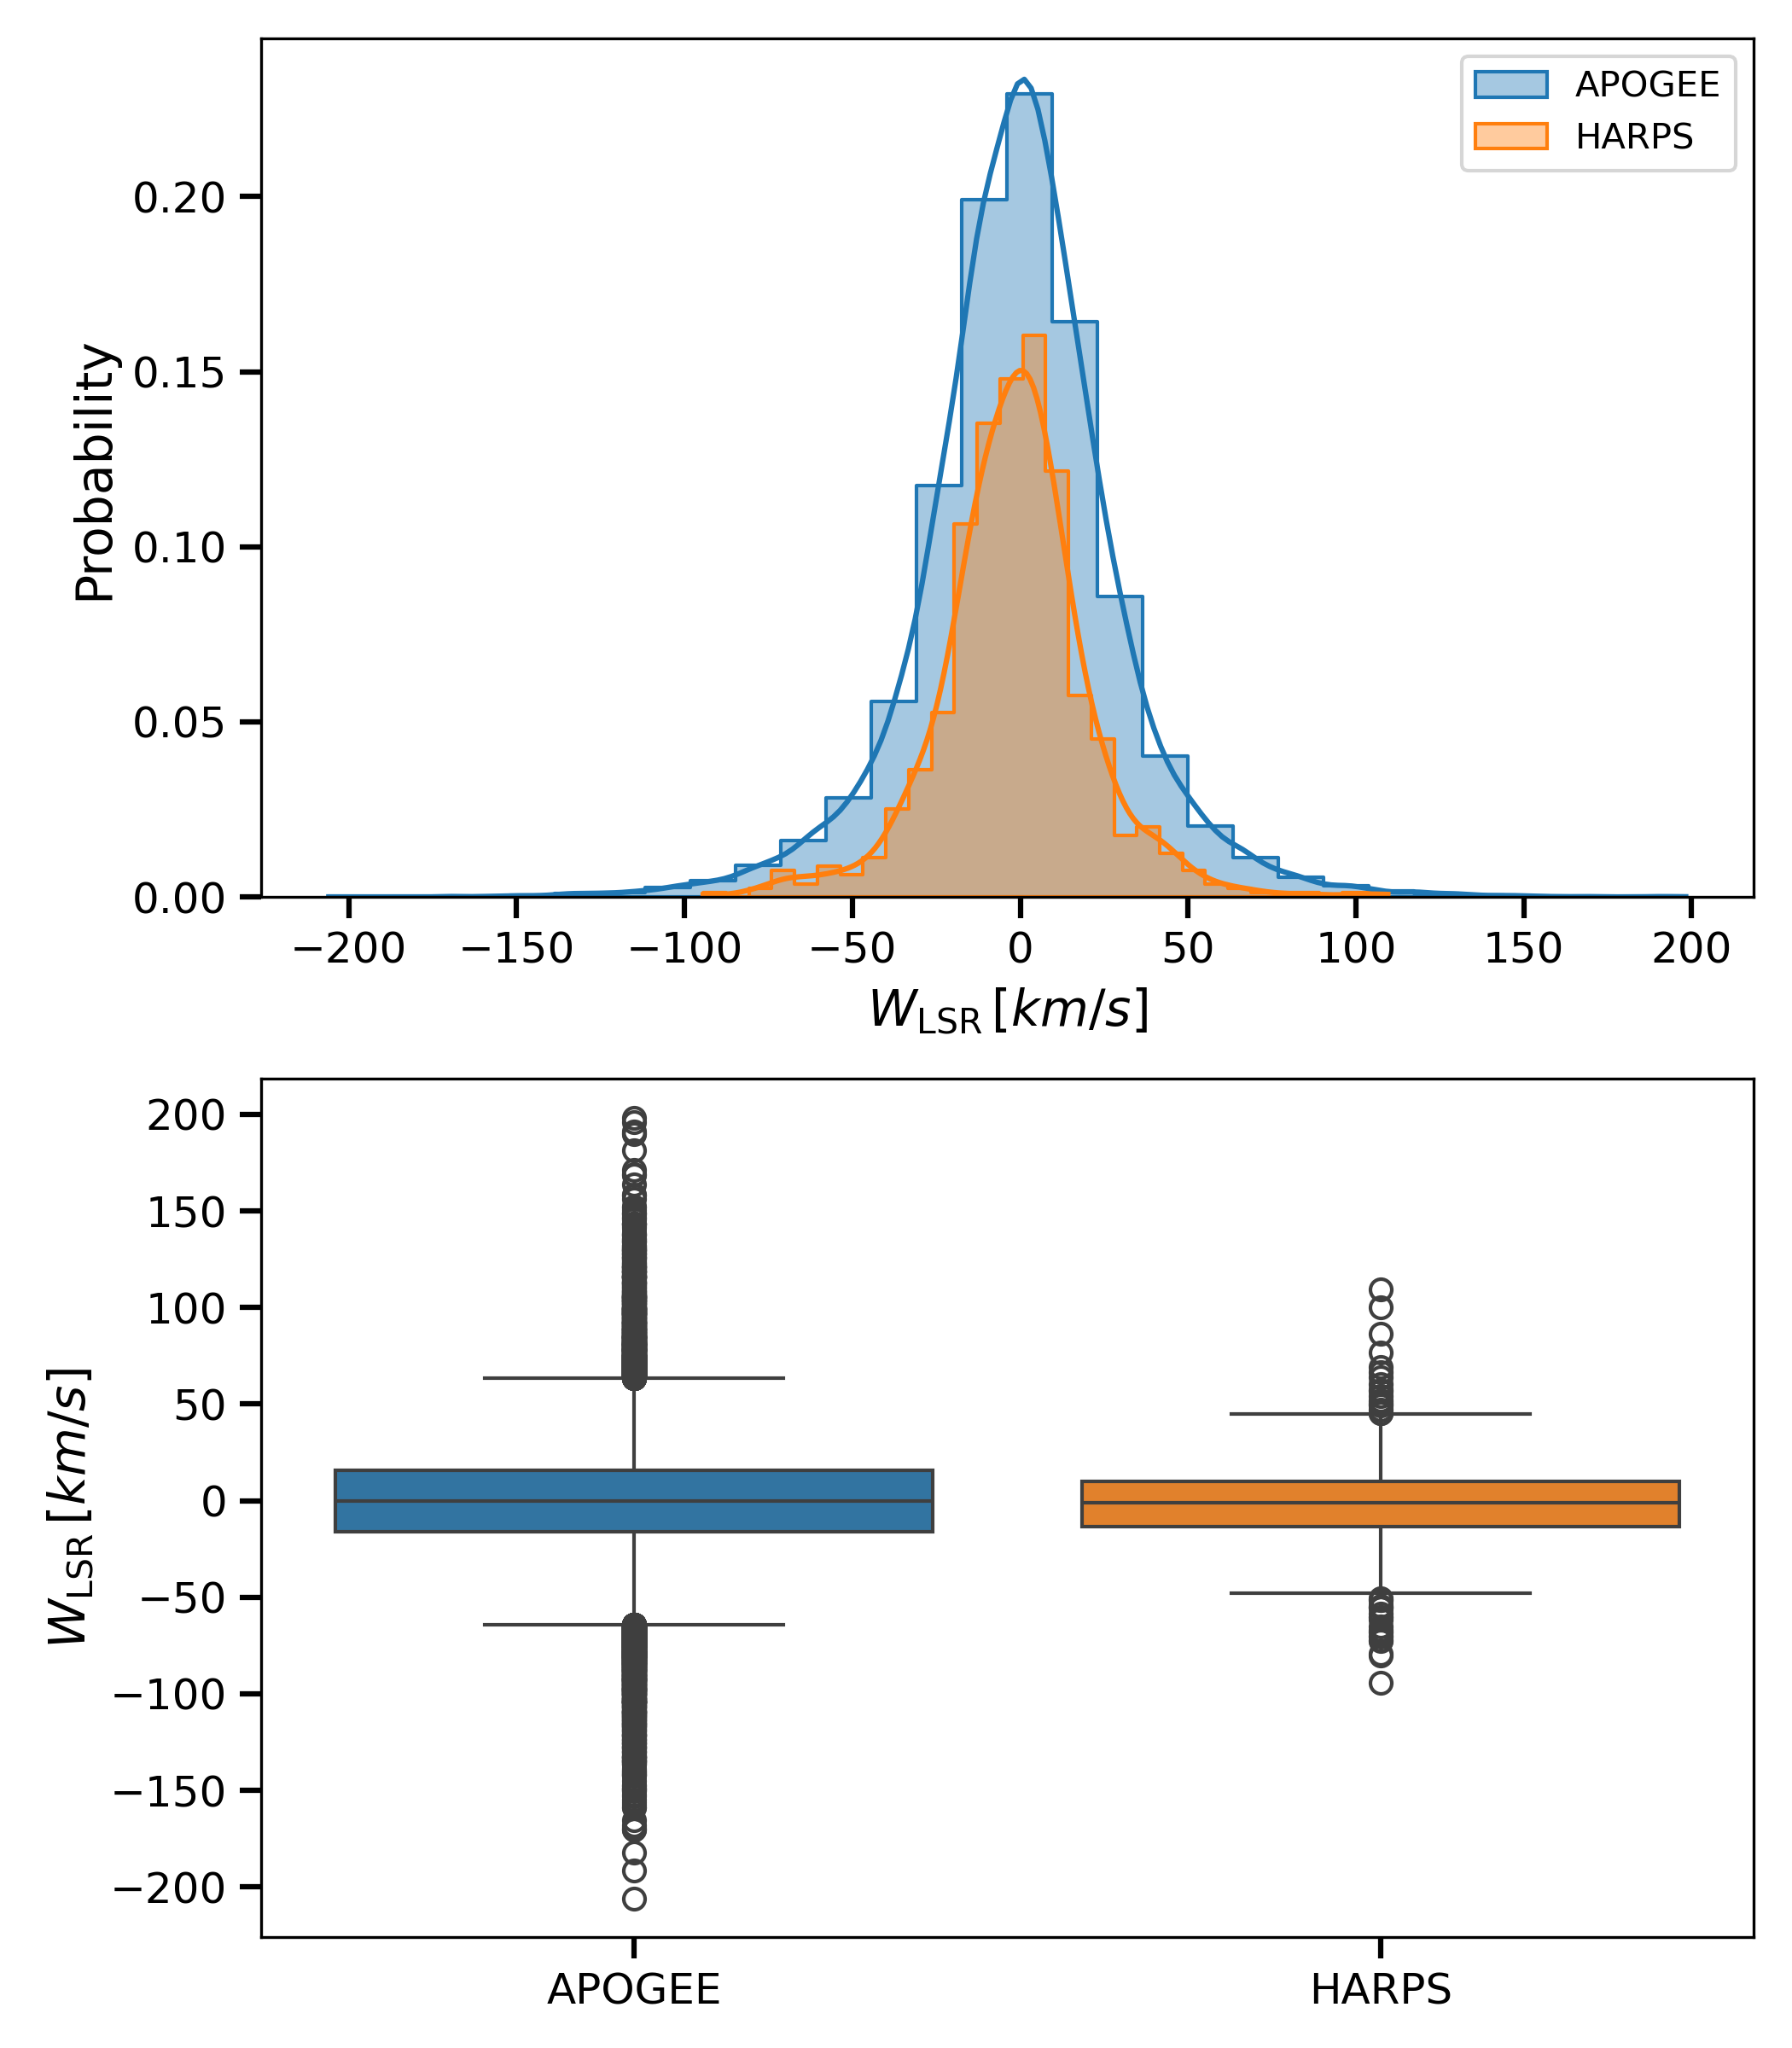
\includegraphics[width=\linewidth]{figures/dist_W_lsr.png}
    \caption{$W_{\mathrm{LSR}}\, [km/s]$}
\end{subfigure}

\vspace{0.4cm}

\begin{subfigure}{0.32\textwidth}
    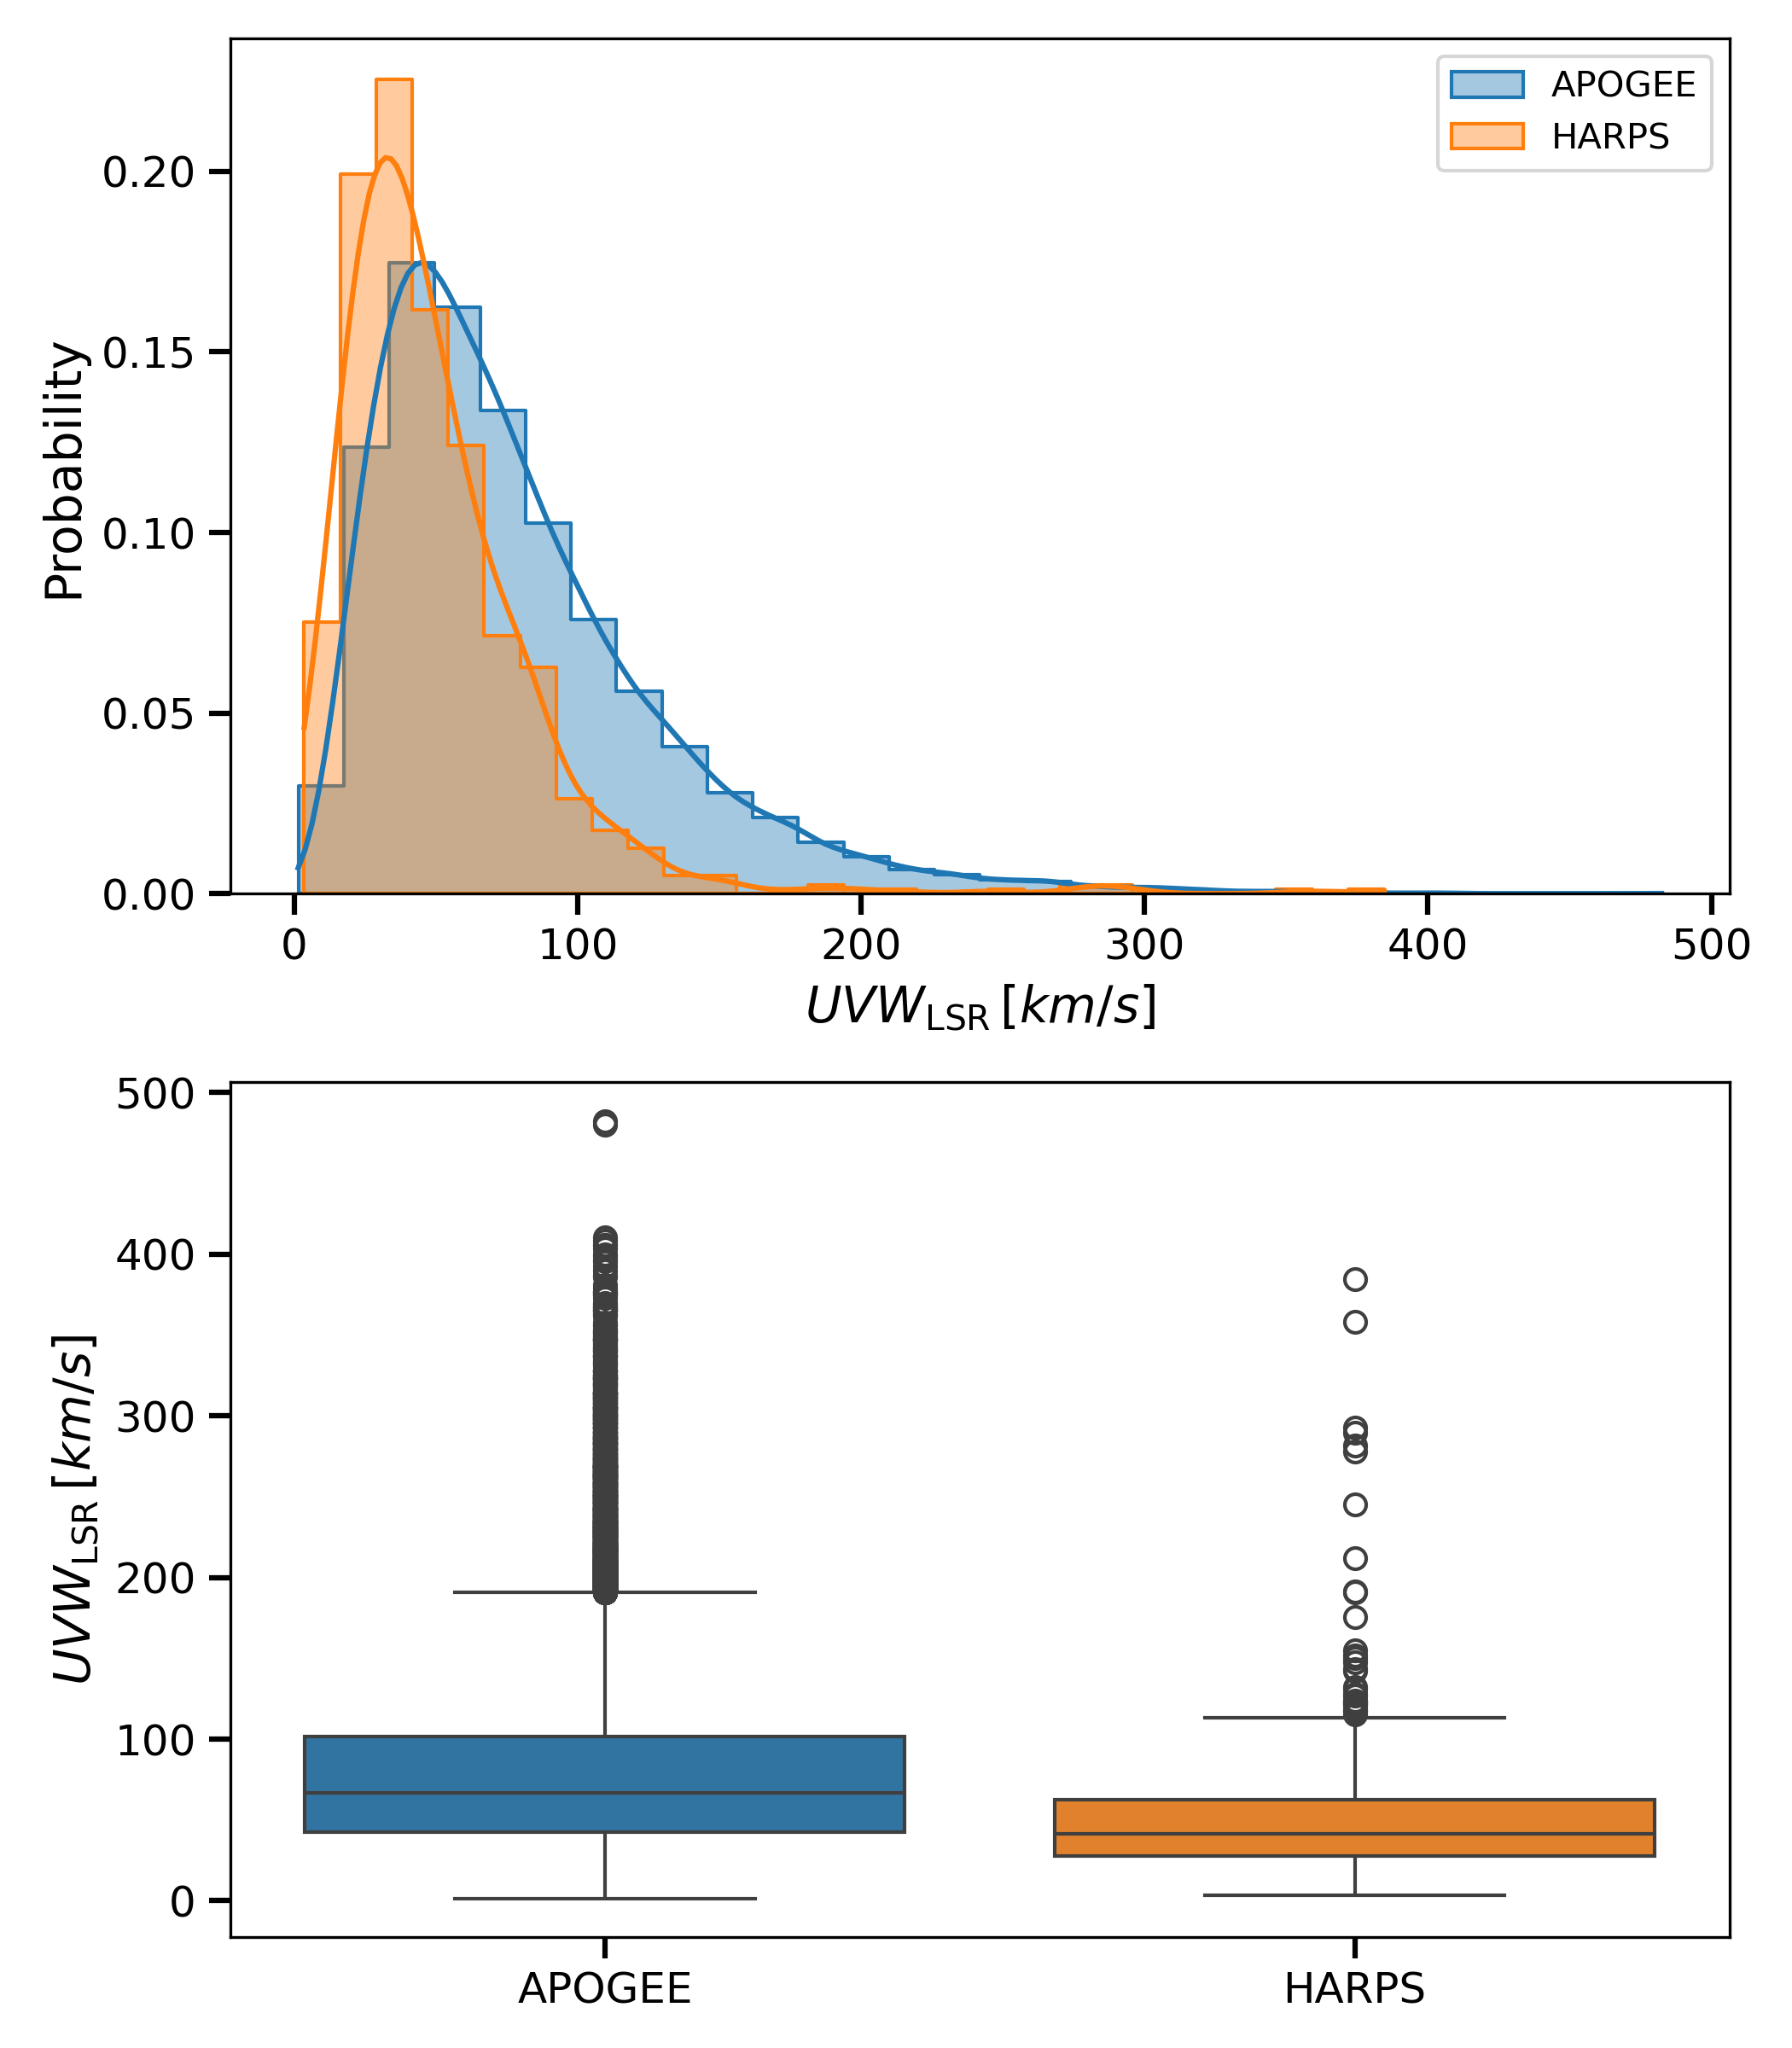
\includegraphics[width=\linewidth]{figures/dist_UVW_lsr.png}
    \caption{$UVW_{\mathrm{LSR}}\, [km/s]$}
\end{subfigure}
\hfill
\begin{subfigure}{0.32\textwidth}
    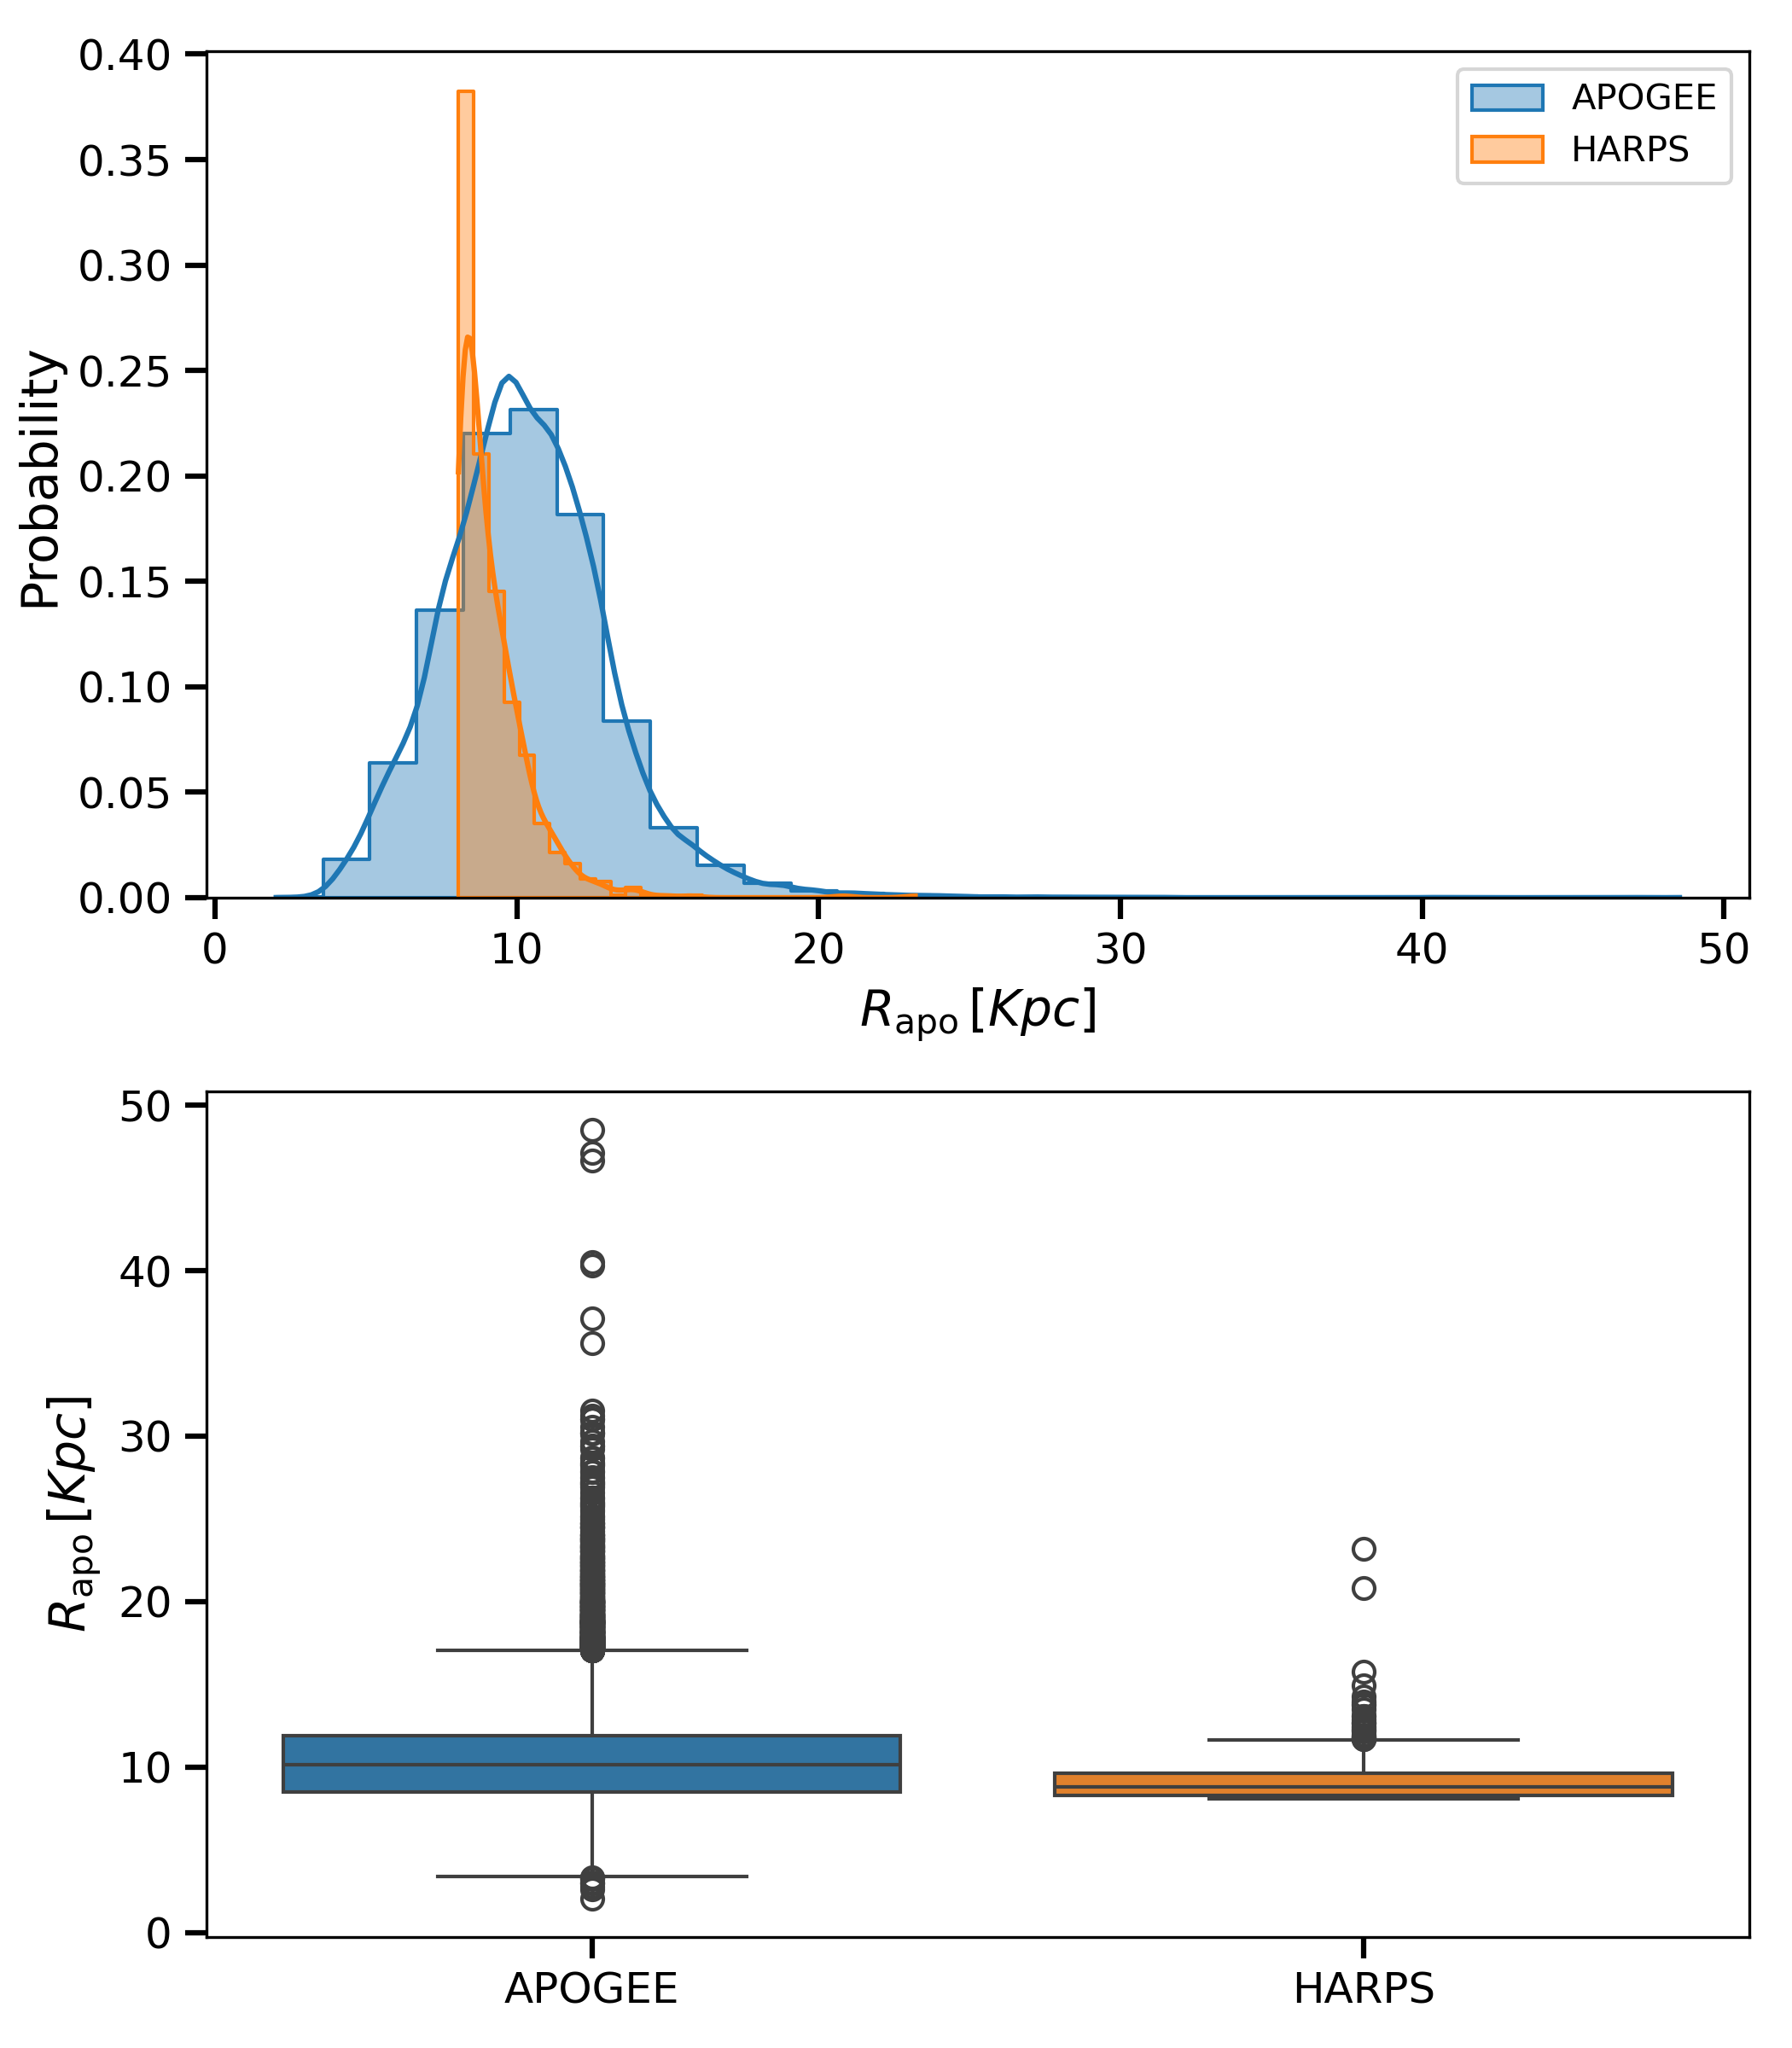
\includegraphics[width=\linewidth]{figures/dist_rapo.png}
    \caption{$R_{\mathrm{apo}}\, [Kpc]$}
\end{subfigure}
\hfill
\begin{subfigure}{0.32\textwidth}
    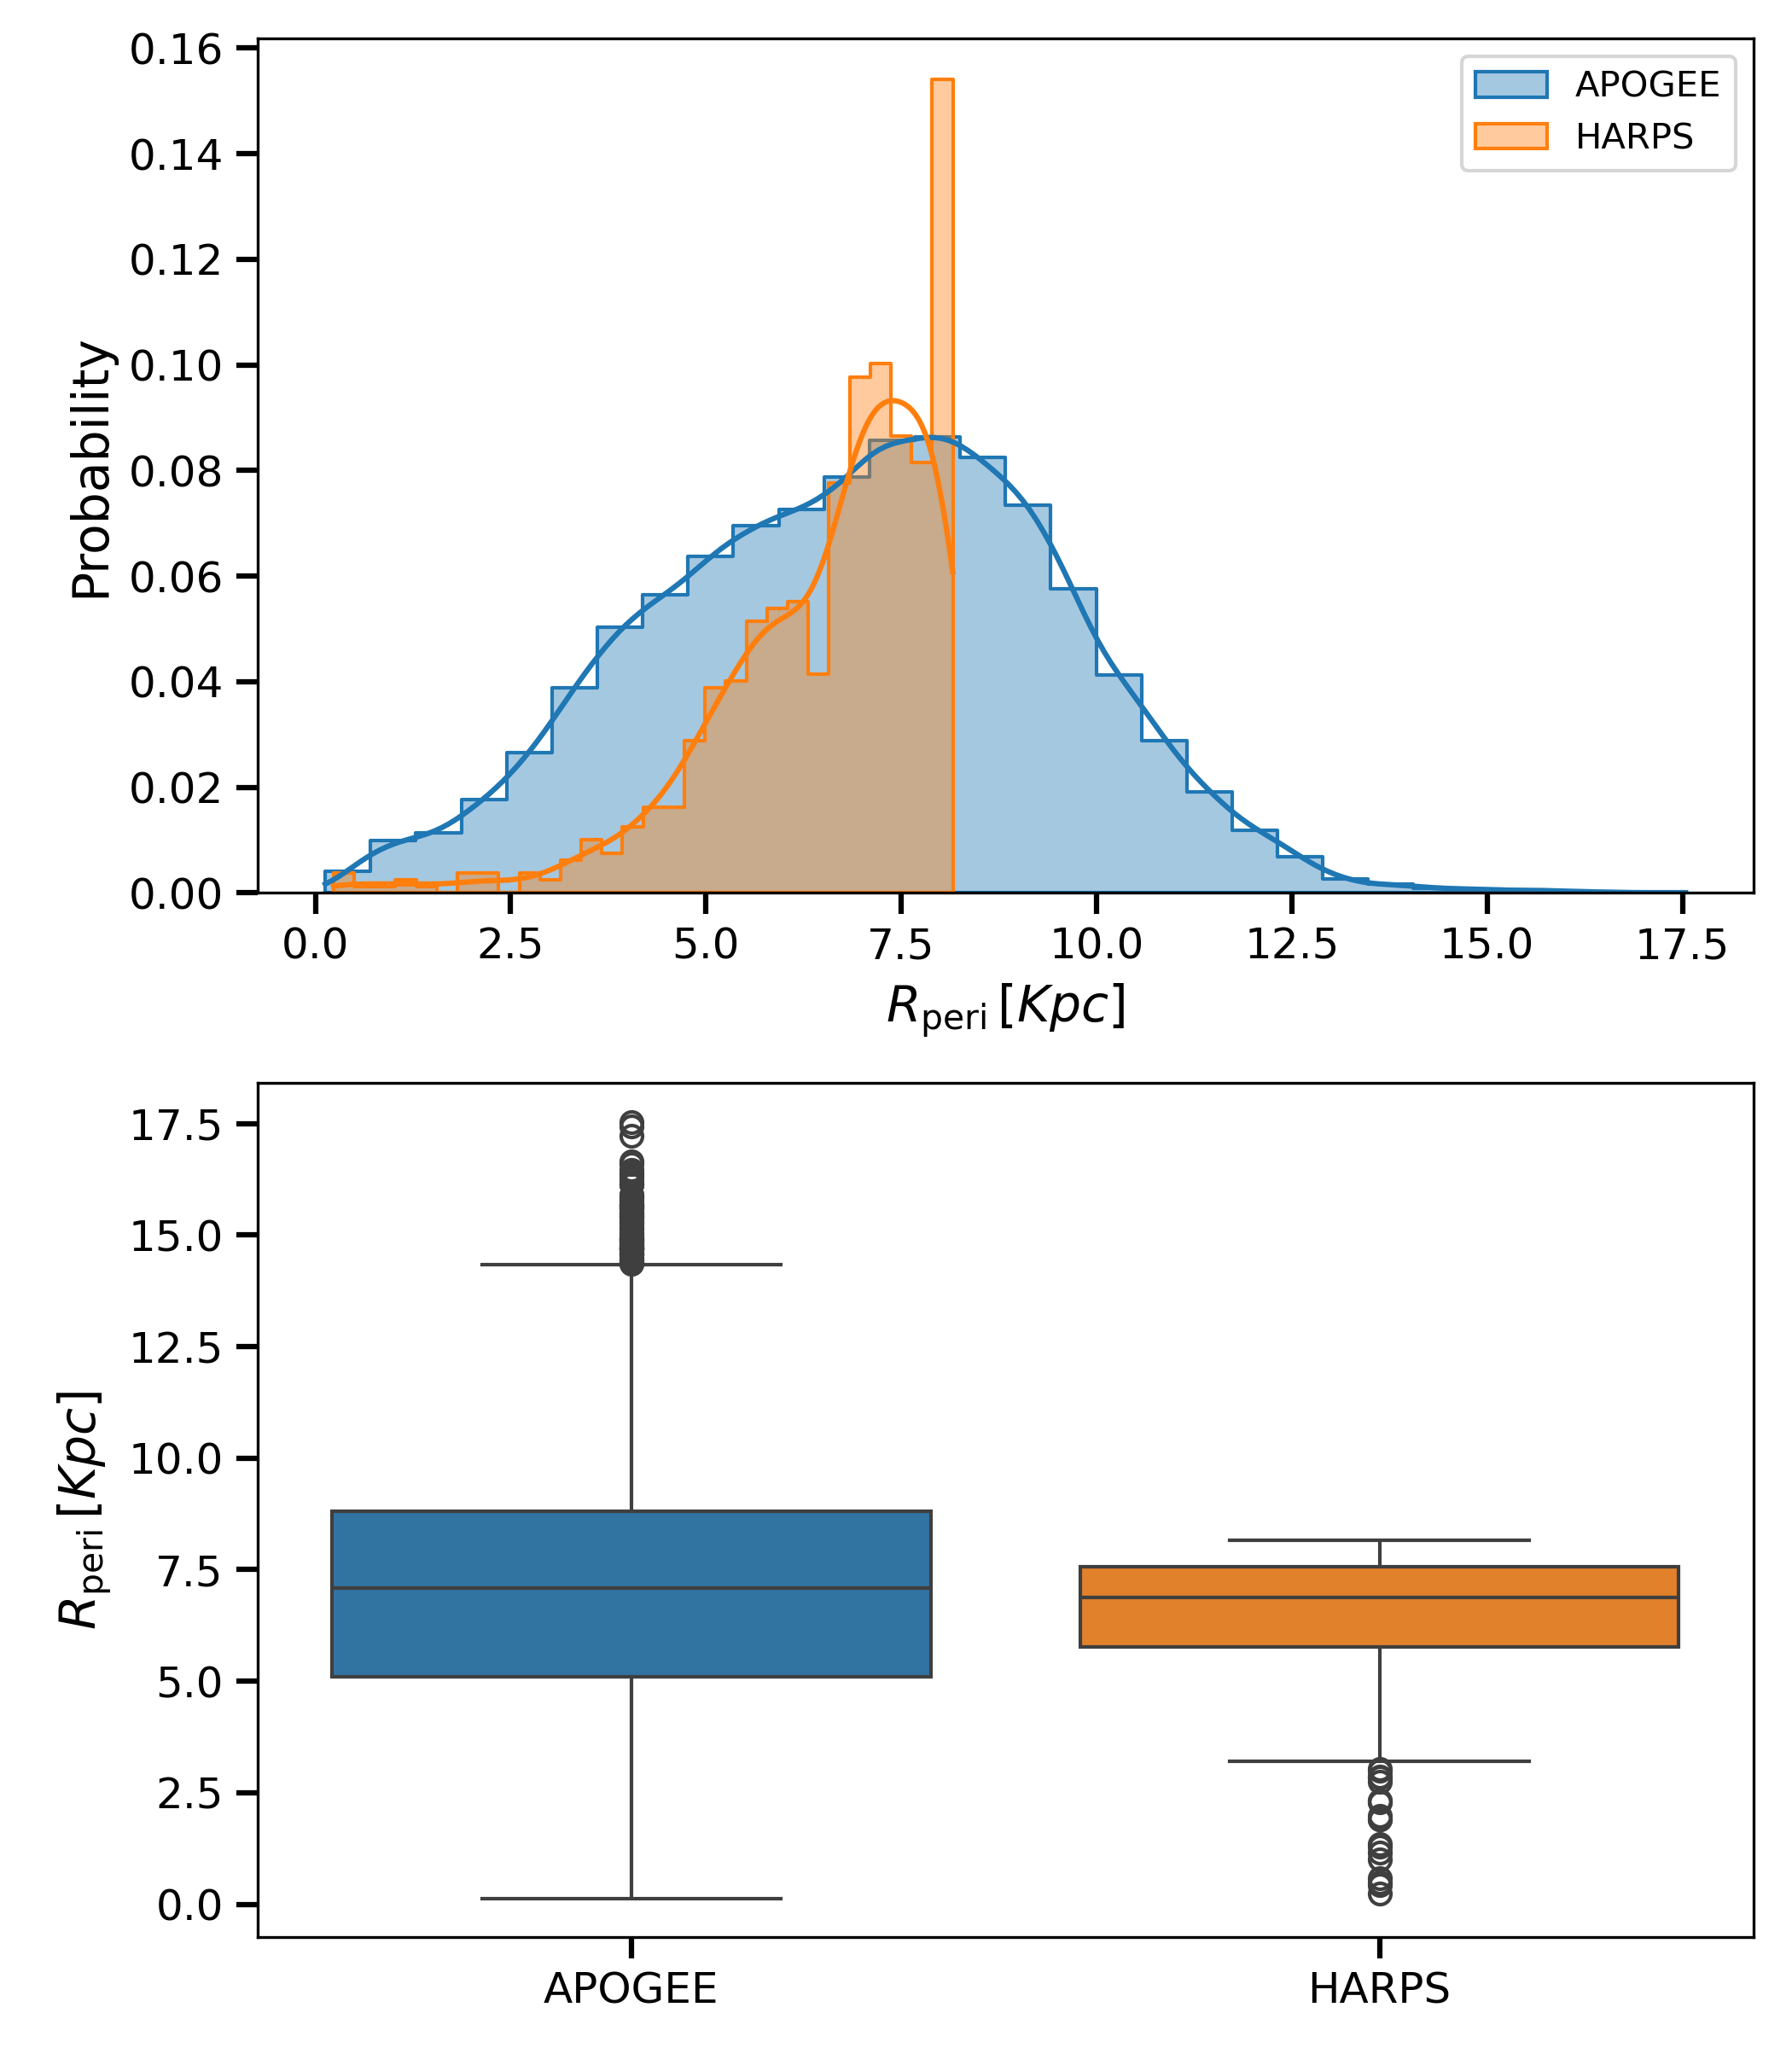
\includegraphics[width=\linewidth]{figures/dist_rperi.png}
    \caption{$R_{\mathrm{peri}}\, [Kpc]$}
\end{subfigure}

\vspace{0.4cm}

\begin{subfigure}{0.32\textwidth}
    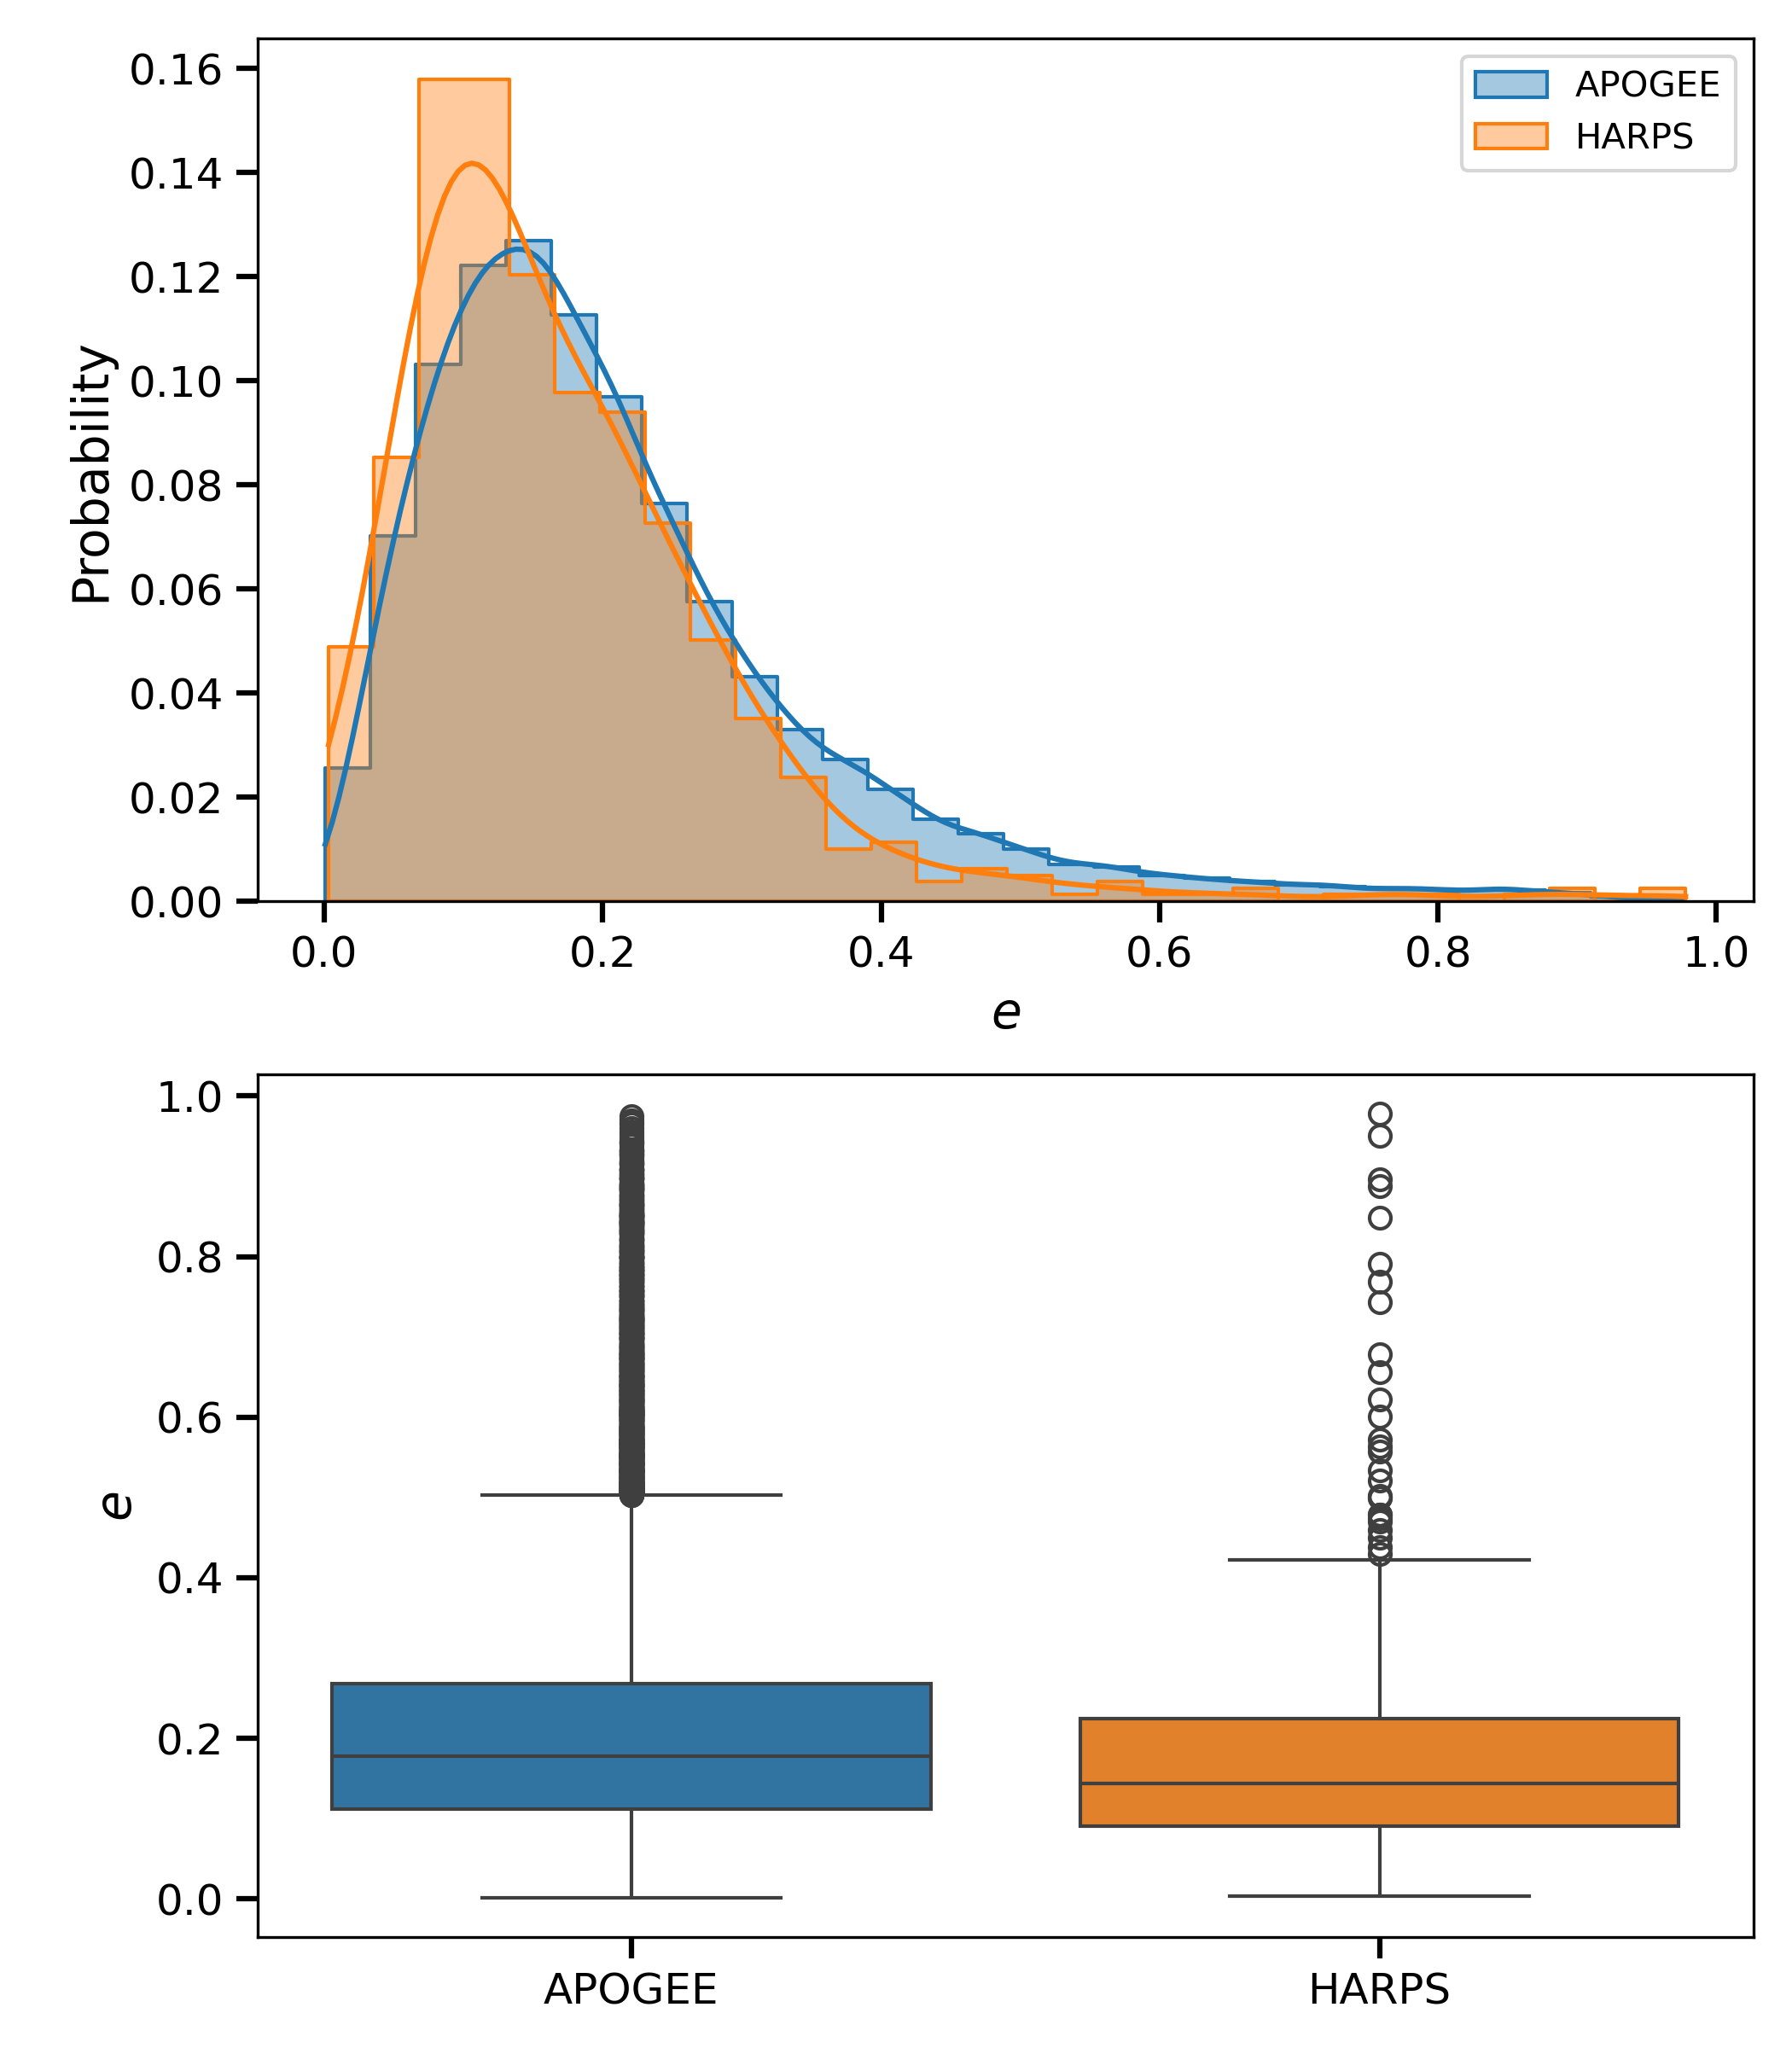
\includegraphics[width=\linewidth]{figures/dist_eccentricity.png}
    \caption{$e$}
\end{subfigure}
\hfill
\begin{subfigure}{0.32\textwidth}
    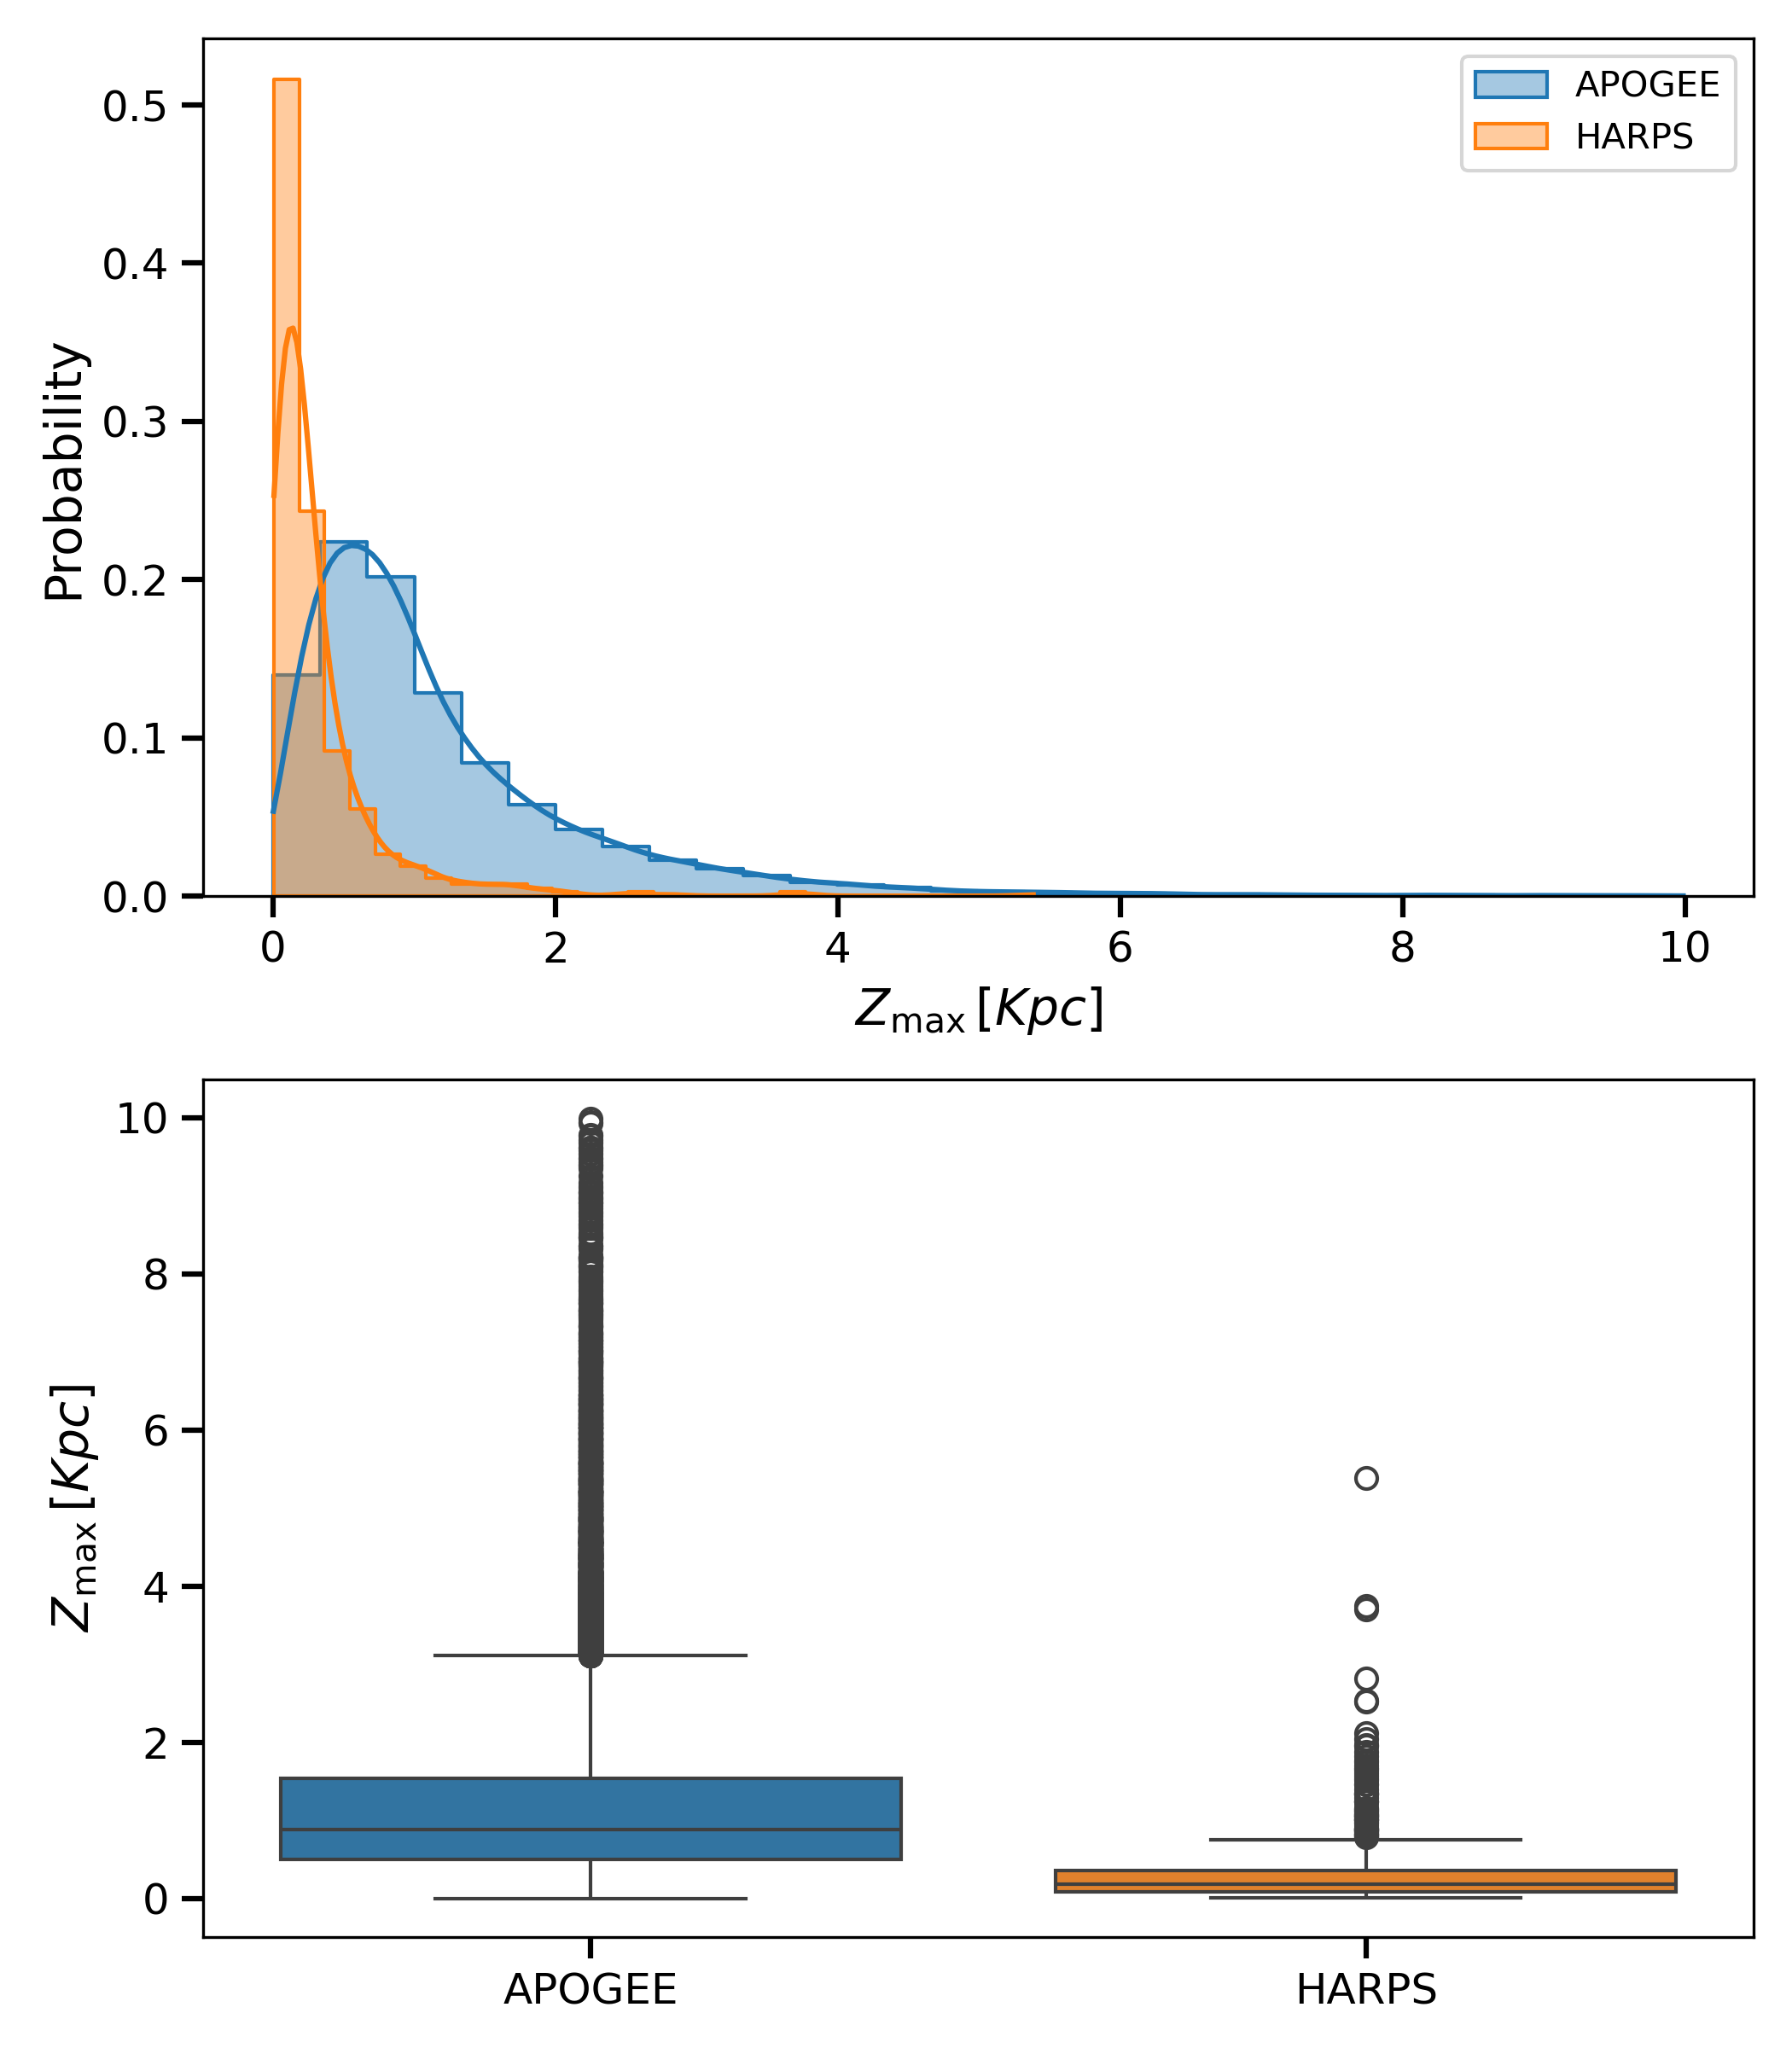
\includegraphics[width=\linewidth]{figures/dist_zmax.png}
    \caption{$Z_{\max}\, [Kpc]$}
\end{subfigure}
\hfill
\begin{subfigure}{0.32\textwidth}
    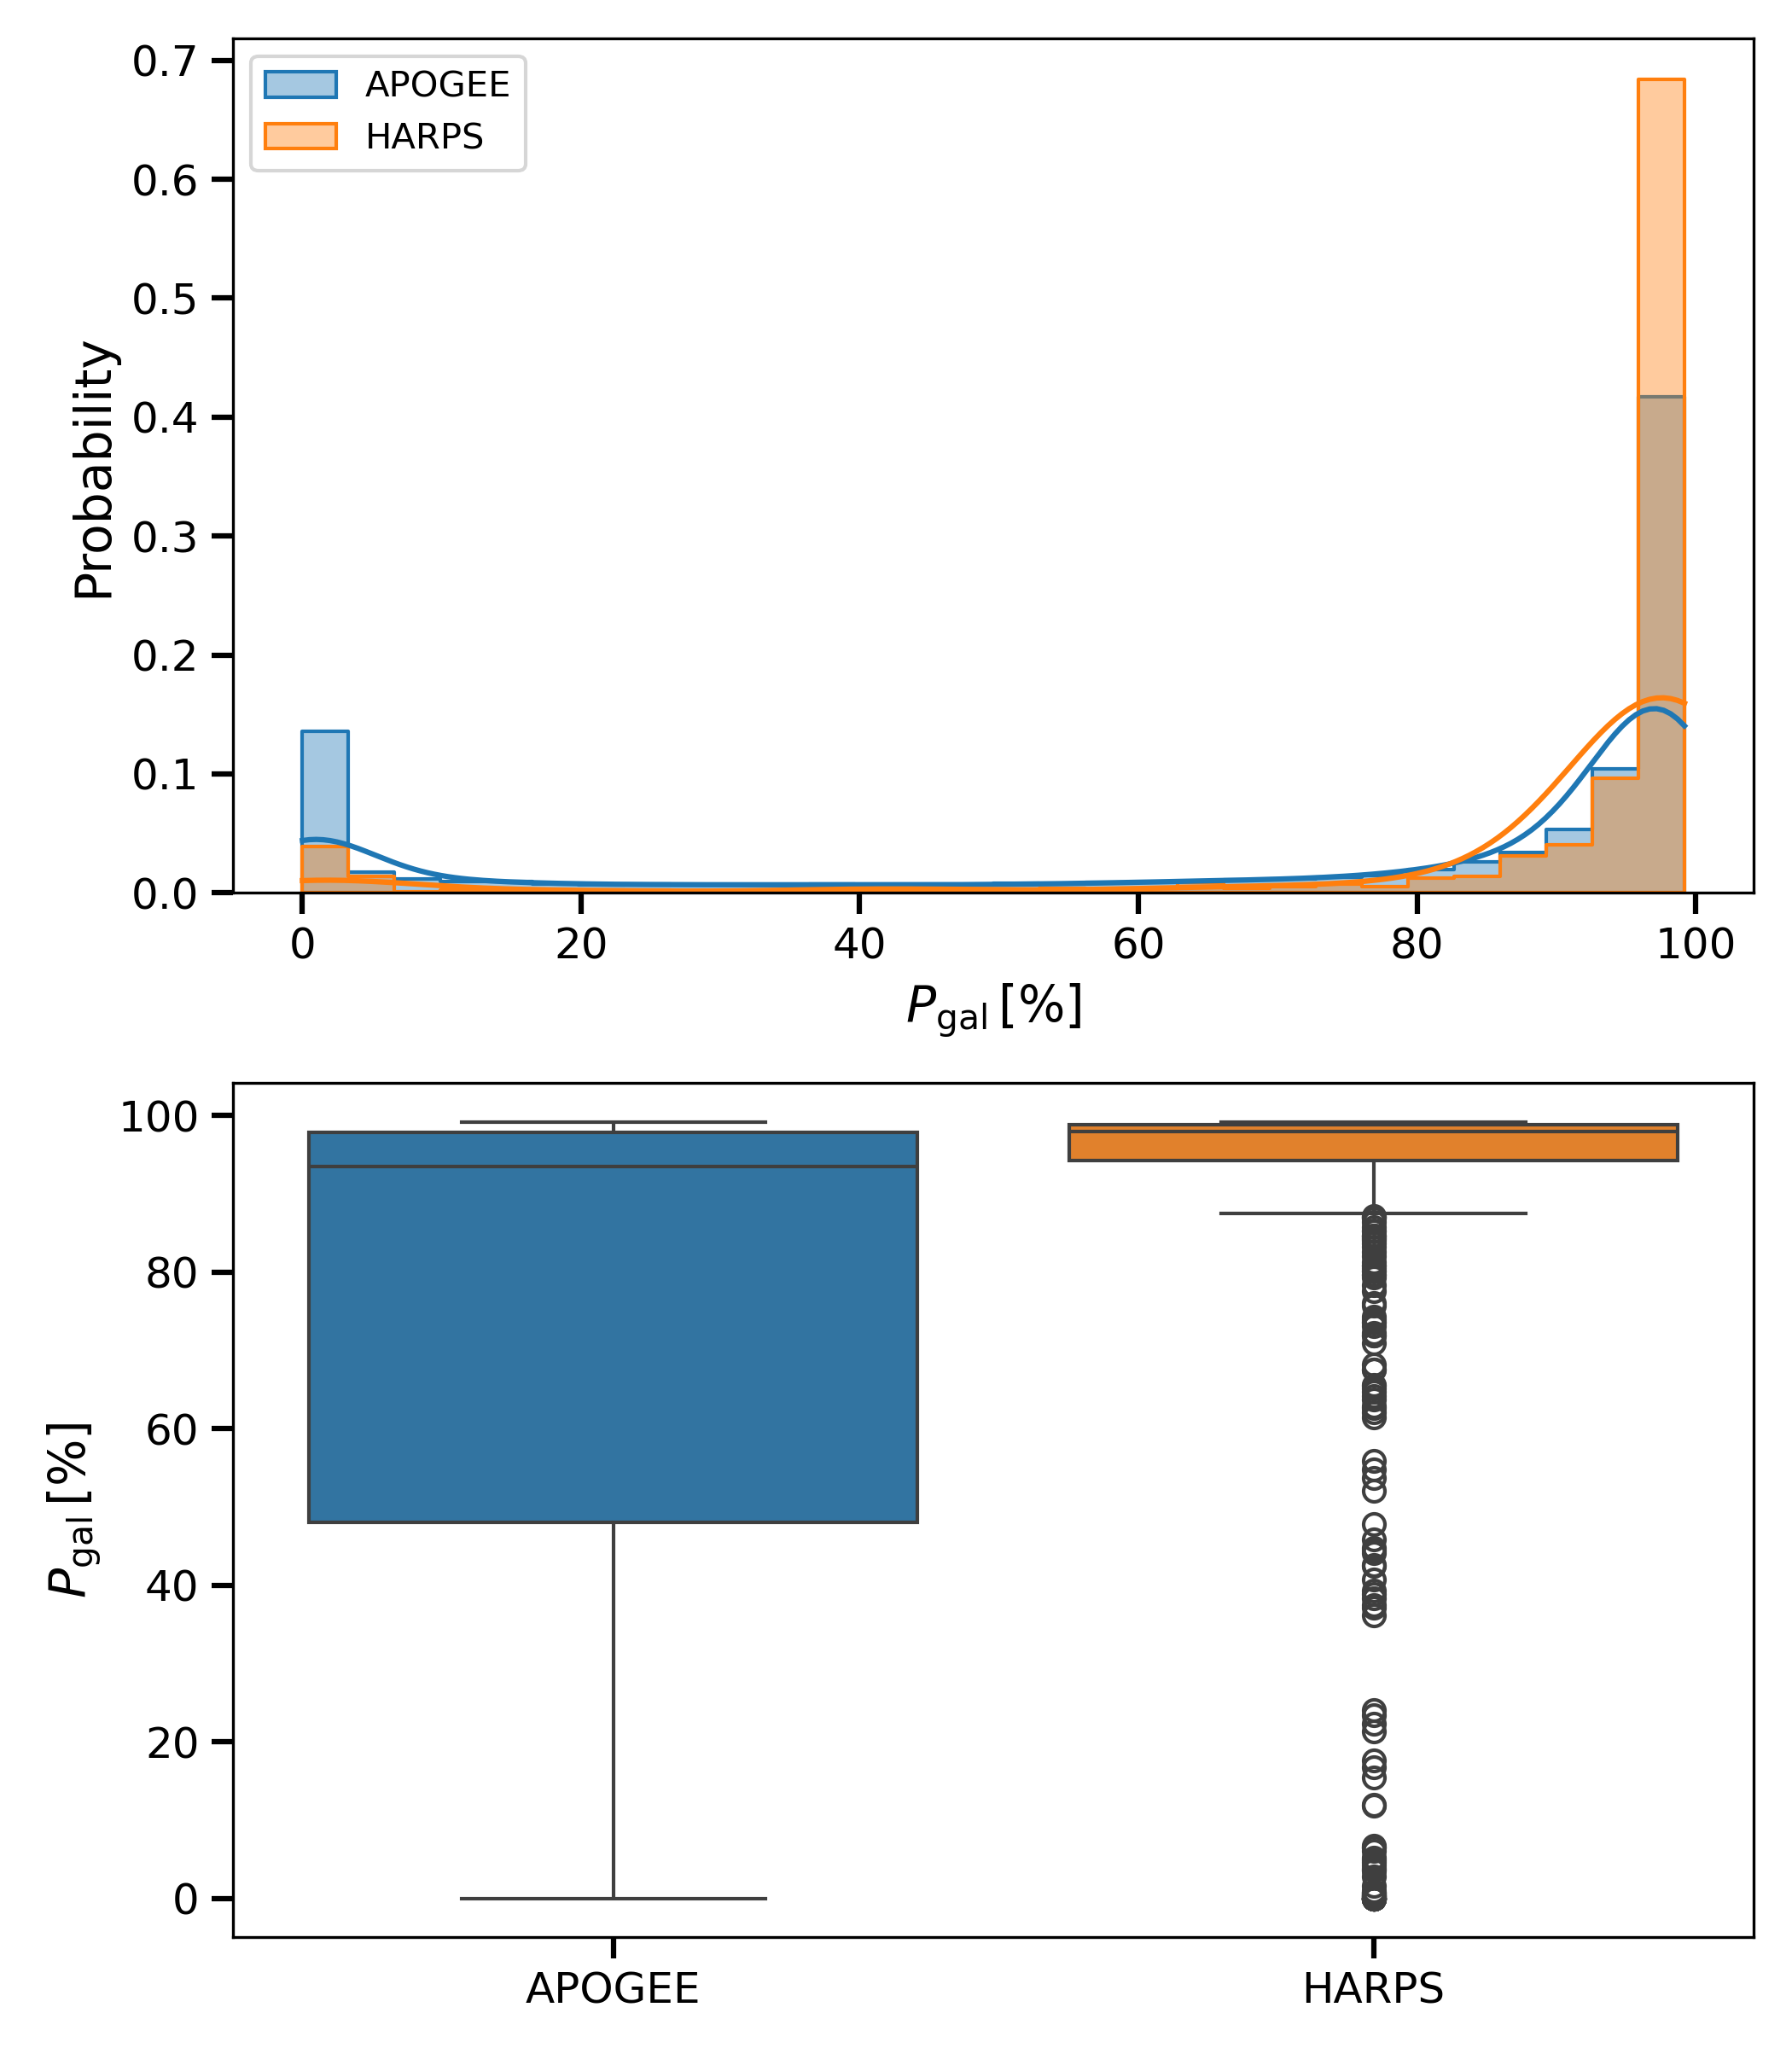
\includegraphics[width=\linewidth]{figures/dist_P_gal.png}
    \caption{$P_{\mathrm{gal}}\, [\%]$}
\end{subfigure}

\caption{Comparison of kinematic and orbital parameters distributions between the APOGEE and HARPS samples. Upper panels show probability-normalized histograms; lower panels show boxplots.}
\label{fig:feature_distributions}
\end{figure*}


\end{appendix}
\end{document}
